%definira klasu dokumenta 
\documentclass[12pt]{report} 

%prostor izmedu naredbi \documentclass i \begin{document} se zove uvod. U njemu se nalaze naredbe koje se odnose na cijeli dokument
	
	%osnovni LaTex ne može riješiti sve probleme, pa se koriste različiti paketi koji olakšavaju izradu željenog dokumenta
	\usepackage[croatian]{babel} 
	\usepackage{amssymb}
	\usepackage{amsmath}
	\usepackage{txfonts}
	\usepackage{mathdots}
	\usepackage{titlesec}
	\usepackage{array}
	\usepackage{lastpage}
	\usepackage{etoolbox}
	\usepackage{tabularray}
	\usepackage{color, colortbl}
	\usepackage{adjustbox}
	\usepackage{geometry}
	\usepackage[classicReIm]{kpfonts}
	\usepackage{hyperref}
	\usepackage{fancyhdr}
		
	\usepackage{float}
	\usepackage{setspace}
	\restylefloat{table}
	
	
	\patchcmd{\chapter}{\thispagestyle{plain}}{\thispagestyle{fancy}}{}{} %redefiniranje stila stranice u paketu fancyhdr
	
	%oblik naslova poglavlja
	\titleformat{\chapter}{\normalfont\huge\bfseries}{\thechapter.}{20pt}{\Huge}
	\titlespacing{\chapter}{0pt}{0pt}{40pt}
	
	
	\linespread{1.3} %razmak između redaka
	
	\geometry{a4paper, left=1in, top=1in,}  %oblik stranice
	
	\hypersetup{ colorlinks, citecolor=black, filecolor=black, linkcolor=black,	urlcolor=black }   %izgled poveznice
	
	
	%prored smanjen između redaka u nabrajanjima i popisima
	\newenvironment{packed_enum}{
		\begin{enumerate}
			\setlength{\itemsep}{0pt}
			\setlength{\parskip}{0pt}
			\setlength{\parsep}{0pt}
		}{\end{enumerate}}
	
	\newenvironment{packed_item}{
		\begin{itemize}
			\setlength{\itemsep}{0pt}
			\setlength{\parskip}{0pt}
			\setlength{\parsep}{0pt}
		}{\end{itemize}}
	
	
	
	
	%boja za privatni i udaljeni kljuc u tablicama
	\definecolor{LightBlue}{rgb}{0.9,0.9,1}
	\definecolor{LightGreen}{rgb}{0.9,1,0.9}
	
	%Promjena teksta za dugačke tablice
	\DefTblrTemplate{contfoot-text}{normal}{Nastavljeno na idućoj stranici}
	\SetTblrTemplate{contfoot-text}{normal}
	\DefTblrTemplate{conthead-text}{normal}{(Nastavljeno)}
	\SetTblrTemplate{conthead-text}{normal}
	\DefTblrTemplate{middlehead,lasthead}{normal}{Nastavljeno od prethodne stranice}
	\SetTblrTemplate{middlehead,lasthead}{normal}
	
	%podesavanje zaglavlja i podnožja
	
	\pagestyle{fancy}
	\lhead{Programsko inženjerstvo}
	\rhead{Digitalni poster}
	\lfoot{Posterheimer}
	\cfoot{stranica \thepage/\pageref{LastPage}}
	\rfoot{\today}
	\renewcommand{\headrulewidth}{0.2pt}
	\renewcommand{\footrulewidth}{0.2pt}
	
	
	\begin{document} 
		
		
		
		\begin{titlepage}
			\begin{center}
				\vspace*{\stretch{1.0}} %u kombinaciji s ostalim \vspace naredbama definira razmak između redaka teksta
				\LARGE Programsko inženjerstvo\\
				\large Ak. god. 2023./2024.\\
				
				\vspace*{\stretch{3.0}}
				
				\huge Digitalni poster\\
				\Large Dokumentacija, Rev. \textit{0.5}\\
				
				\vspace*{\stretch{12.0}}
				\normalsize
				Grupa: \textit{Posterheimer}\\
				Voditelj: \textit{Dominik Papeš}\\
				
				
				\vspace*{\stretch{1.0}}
				Datum predaje: \textit{17. 11. 2023.}\\
				
				\vspace*{\stretch{4.0}}
				
				Nastavnik: \textit{Miljenko Krhen}\\
				
			\end{center}
			
			
		\end{titlepage}
		
		
		\tableofcontents
		
		
		\chapter{Dnevnik promjena dokumentacije}		
		
		\begin{longtblr}[
				label=none
			]{
				width = \textwidth, 
				colspec={|X[2]|X[13]|X[3]|X[3]|}, 
				rowhead = 1
			}
			\hline
			\textbf{Rev.}	& \textbf{Opis promjene/dodatka} & \textbf{Autori} & \textbf{Datum}\\[3pt] \hline
			0.1 & Napravljen predložak.	& {\small V. Javornik} & 22.10.2023. 		\\[3pt] \hline 
			0.2	& Dodan osnovni opis projektnog zadatka & {\small V. Javornik} &23.10.2023.  \\[3pt] \hline 
			0.2.1 & Manje promjene opisa projektnog zadatka & {\small V. Javornik} &  24.10.2023.\\ [3pt] \hline
			0.2.2 & Ažuriran dnenvnik sastajanja & {\small V. Javornik} &  24.10.2023.\\ [3pt] \hline
			0.3 & Dodani aktori & {\small D. Papeš} & 24.10.2023.\\ [3pt] \hline
			0.3.1 & Dopunjeni aktori & {\small D. Papeš} & 25.10.2023.\\ [3pt] \hline
			0.4 & Pobrojani funkcionalni zahtjevi & {\small D. Papeš} & 25.10.2023.\\ [3pt] \hline
			0.4.1 & Opisani obrasci uporabe 2-5 & {\small F. Androić} & 26.10.2023.\\ [3pt] \hline
			0.4.2 & Male jezične promjene, dopunjeni aktori & {\small F. Androić} & 26.10.2023.\\ [3pt] \hline
			0.4.3 & Dodan prvi dio opisa obrazaca uporabe & {\small V.Javornik } & 26.10.2023. \\ [3pt] \hline
			0.4.4 & Definirani obrasci uporabe 6-9, 14-17 i 30, dodani nefunkcionalni zahtjevi, ažuriran opis projektnog zadatka & {\small M. Perhat } & 26.10.2023. \\ [3pt] \hline
			0.4.5 & Definirani obrasci uporabe 22-26 & {\small D. Papeš } & 27.10.2023. \\ [3pt] \hline
			0.4.6 & Definirani obrasci uporabe 12-14 & {\small D. Tomšić } & 27.10.2023. \\ [3pt] \hline
			0.4.7 & Definirani obrasci uporabe 19 i 20, pobrisan obrazac uporabe 21 (Uređivanje digitalnog postera) & {\small F. Androić } & 27.10.2023. \\ [3pt] \hline
			0.5 & Dodan početni dijagram obrazaca uporabe & {\small F. Androić } & 27.10.2023. \\ [3pt] \hline
			0.5.1 & Ažuriran opis i ostali zahtjevi & {\small D. Papeš} & 1.11.2023. \\ [3pt] \hline
			0.5.2 & Ažurirani obrasci uporabe & {\small D. Papeš} & 1.11.2023. \\ [3pt] \hline
			0.5.3 & Ažurirani obrasci uporabe & {\small D. Papeš} & 4.11.2023. \\ [3pt] \hline
			0.6 & Dodan sekvencijski dijagram za upravljanje digitalnim posterima & {\small V. Javornik} & 4.11.2023. \\ [3pt] \hline
			0.6.1 & Ažuriran popis aktora, dodani dijagrami obrazaca uporabe za opis korisničkih računa i za administratorove i natkorisnikove mogućnosti, uklonjen početni dijagram obrazaca uporabe & {\small F. Androić} & 4.11.2023. \\ [3pt] \hline
			0.6.2 & Dodan dijagram obrazaca uporabe za opis funkcionalnosti aplikacije, manje
			jezične promjene & {\small D. Tomšić} & 5.11.2023. \\ [3pt] \hline
			0.6.3 & Dodan sekvencijski dijagram za slanje e-pošte & {\small M. Perhat} & 5.11.2023. \\ [3pt] \hline
			0.6.4 & Dodan sekvencijski dijagram za glasanje & {\small D. Papeš} & 6.11.2023. \\ [3pt] \hline
			0.7 & Dodan opis tablica i dijagram baze podataka & {\small V. Javornik} & 9.11.2023. \\ [3pt] \hline
			0.7.1 & Dopunjen opis projektnog zadatka, izbrisane smjernice za 1. reviziju, dodan dijagram razreda, gramatički ispravci & {\small F. Androić} & 13.11.2023. \\ [3pt] \hline
			0.7.2 & Napisan opis dijagrama razreda, dodan Dijagram razreda - dio Controllers & {\small V. Javornik} & 14.11.2023. \\ [3pt] \hline
			0.7.3 & Dodan dijagram razreda, ažuriran dnevnik sastajanja, male jezične promjene & {\small D. Tomšić} & 14.11.2023. \\ [3pt] \hline
			0.7.4 & Izmjene opisa projektnog zadatka, izmjene obrazaca uporabe (Upravljanje podacima o konferenciji i Poziv na dodjelu nagrade), izmjene UC dijagrama, izmjene opisa dijagrama razreda & {\small F. Androić} & 14.11.2023. \\ [3pt] \hline
			0.8 & Dodan opis arhitekture i dizajna sustava & {\small A. Batić} & 14.11.2023. \\ [3pt] \hline
			0.8.1 & Uređen opis arhitekture i dodana slika, ažuriran dnevnik sastanaka & {\small F. Androić} & 14.11.2023. \\ [3pt] \hline
			0.8.2 & Usklađivanje opisa baze podataka sa stvarnom implementacijom & {\small V. Javornik} & 16.11.2023. \\ [3pt] \hline
		\end{longtblr}
		\chapter{Opis projektnog zadatka}
		
		\textbf{\textit{dio 1. revizije}}\\
		
		\textit{Na osnovi projektnog zadatka detaljno opisati korisničke zahtjeve. Što jasnije opisati cilj projektnog zadatka, razraditi problematiku zadatka, dodati nove aspekte problema i potencijalnih rješenja. Očekuje se minimalno 3, a poželjno 4-5 stranica opisa.	Teme koje treba dodatno razraditi u ovom poglavlju su:}
		\begin{packed_item}
			\item \textit{potencijalna korist ovog projekta}
			\item \textit{postojeća slična rješenja (istražiti i ukratko opisati razlike u odnosu na zadani zadatak). Dodajte slike koja predočavaju slična rješenja.}
			\item \textit{skup korisnika koji bi mogao biti zainteresiran za ostvareno rješenje.}
			\item \textit{mogućnost prilagodbe rješenja }
			\item \textit{opseg projektnog zadatka}
			\item \textit{moguće nadogradnje projektnog zadatka}
		\end{packed_item}
		
		\textit{Za pomoć pogledati reference navedene u poglavlju „Popis literature“, a po potrebi konzultirati sadržaj na internetu koji nudi dobre smjernice u tom pogledu.}
		\eject
		

		\chapter{Specifikacija programske potpore}
		
	\section{Funkcionalni zahtjevi}
			
			\textbf{\textit{dio 1. revizije}}\\
			
			\textit{Navesti \textbf{dionike} koji imaju \textbf{interes u ovom sustavu} ili  \textbf{su nositelji odgovornosti}. To su prije svega korisnici, ali i administratori sustava, naručitelji, razvojni tim.}\\
				
			\textit{Navesti \textbf{aktore} koji izravno \textbf{koriste} ili \textbf{komuniciraju sa sustavom}. Oni mogu imati inicijatorsku ulogu, tj. započinju određene procese u sustavu ili samo sudioničku ulogu, tj. obavljaju određeni posao. Za svakog aktora navesti funkcionalne zahtjeve koji se na njega odnose.}\\
			
			
			\noindent \textbf{Dionici:}
			
			\begin{packed_enum}
				
				\item Organizator konferencije (naručitelj)
				\item Pokrovitelji konferencije
				\item Autori radova
				\item Glasači
				\item Administrator
				\item Razvojni tim
				
			\end{packed_enum}
			
			\noindent \textbf{Aktori i njihovi funkcionalni zahtjevi:}
			
			\begin{packed_enum}
				\item  \underbar{Neregistrirani/Neprijavljeni korisnik (inicijator) može:}
				
				\begin{packed_enum}
					
					\item upisati lozinku za konferenciju
					\item registrirati se to jest stvoriti novi korisnički račun za koji su mu potrebni: korisničko ime, lozinka i adresa e-pošte
					\item prijaviti se
					\item pregledavati postere, pri čemu ne može glasati
					
				\end{packed_enum}
			
				\item  \underbar{Registrirani/Prijavljeni korisnik (inicijator) može:}
				
				\begin{packed_enum}
					
					\item pregledavati i mijenjati osobne podatke
					\item izbrisati svoj korisnički račun
					\item pregledavati i glasati za postere pri čemu svaki posjetitelj može glasati najviše za jedan poster
					\item pregledavati promotivne materijale pokrovitelja
					\item gledati video-prijenos
					\item pregledavati i preuzimati fotografije
					\item vidjeti informacije o mjestu održavanja koje uključuju vremenske uvjete i vremensku prognozu
					\item pristupiti rezultatima jednom kad postanu dostupni
				
				\end{packed_enum}
				
				\item \underbar{Administrator (inicijator) može:}
				
				\begin{packed_enum}
					
					\item prijaviti i ukloniti autore, radove i postere
					\item pristupiti svim podacima
					\item definirati sve uvjete za rad sustava
					
				\end{packed_enum}
				
				\item \underbar{Baza podataka (sudionik):}
				
				\begin{packed_enum}
					
					\item pohranjuje podatke o korisnicima
					\item pohranjuje podatke o digitalnim posterima, broju njihovih glasova, njihovim autorima
					\item pohranjuje fotografije uslikane za vrijeme trajanja konferencije
					
				\end{packed_enum}
				
				\item \underbar{Poslužitelj strujanja (sudionik):}
				
				\begin{packed_enum}
					
					\item pruža uslugu video prijenosa konferencije
				
				\end{packed_enum}
				
				\item \underbar{Poslužitelj podataka o vremenu (sudionik):}
				
				\begin{packed_enum}
					
					\item poslužuje potrebne podatke vezane za prognozu vremena
					
				\end{packed_enum}
				
				\item \underbar{Poslužitelj e-pošte (sudionik):}
				
				\begin{packed_enum}
					
					\item omogućuje aplikaciji da šalje e-poruke korisnicima
					
				\end{packed_enum}
				
			\end{packed_enum}
			
			\eject 
			
			
				
			\subsection{Obrasci uporabe}
				
				\textbf{\textit{dio 1. revizije}}
				
				\subsubsection{Opis obrazaca uporabe}
					\textit{Funkcionalne zahtjeve razraditi u obliku obrazaca uporabe. Svaki obrazac je potrebno razraditi prema donjem predlošku. Ukoliko u nekom koraku može doći do odstupanja, potrebno je to odstupanje opisati i po mogućnosti ponuditi rješenje kojim bi se tijek obrasca vratio na osnovni tijek.}\\
					
					\newcounter{UseCaseCounter}
					\setcounter{UseCaseCounter}{1}
					
					%UC1
					\noindent \underbar{\textbf{UC\theUseCaseCounter \stepcounter{UseCaseCounter} - Pristup konferenciji}}
					\begin{packed_item}
	
						\item \textbf{Glavni sudionik: } Neprijavljeni korisnik
						\item  \textbf{Cilj:} Pristup konferenciji
						\item  \textbf{Sudionici:} Baza podataka
						\item  \textbf{Preduvjet:} Korisnik već nije prijavljen
						\item  \textbf{Opis osnovnog tijeka:}
						
						\item[] \begin{packed_enum}
	
							\item Korisnik pokreće aplikaciju
							\item Pojavljuje se obrazac za upis lozinke za pristup konferenciji (isti je za sve korisnike za tu konferenciju)
							\item Korisnik upiše lozinku te ju potvrđuje
							\item Obrazac za upis lozinke nestaje i pojavljuje se ekran s prikazom svih postera
						\end{packed_enum}
						
						\item  \textbf{Opis mogućih odstupanja:}
						
						\item[] \begin{packed_item}
	
							\item[3.a] Korisnik upiše krivu lozinku
							\item[] \begin{packed_enum}
								
								\item Pristup pregledu konferencije je odbijen
								\item Sustav obavještava korisnika o upisu pogrešne lozinke ili imena
								
							\end{packed_enum}
							
						\end{packed_item}
					\end{packed_item}
					
					%UC2
					\noindent \underbar{\textbf{UC\theUseCaseCounter \stepcounter{UseCaseCounter} - Prijava}}
					\begin{packed_item}
						
						\item \textbf{Glavni sudionik: } Neprijavljeni korisnik
						\item  \textbf{Cilj:} Pristup svim korisničkim funkcionalnostima aplikacije
						\item  \textbf{Sudionici:} Baza podataka
						\item  \textbf{Preduvjet:} Korisnik je registriran
						\item  \textbf{Opis osnovnog tijeka:}
						
						\item[] \begin{packed_enum}
							
							\item Korisnik pritišće gumb za prijavu na početnoj stranici
							\item Otvara se novi prozor u koji korisnik upisuje podatke
							\item Provjera postoji li korisnik u bazi podataka
							\item Ako korisnik postoji, otvara se prozor s posterima, a korisnik je prijavljen
						\end{packed_enum}
						
						\item  \textbf{Opis mogućih odstupanja:}
						
						\item[] \begin{packed_item}
							
							\item[4.a] Korisnik ne postoji u bazi podataka
							\item[] \begin{packed_enum}
								
								\item Sustav obavještava korisnika o upisu pogrešne lozinke ili imena
								
							\end{packed_enum}
							
						\end{packed_item}
					\end{packed_item}	
					
					%UC3
					\noindent \underbar{\textbf{UC\theUseCaseCounter \stepcounter{UseCaseCounter} - Registracija}}
					\begin{packed_item}
					
						\item \textbf{Glavni sudionik: } Neprijavljeni korisnik
						\item  \textbf{Cilj:} Stvoriti korisnički račun za pristup sustavu
						\item  \textbf{Sudionici:} Baza podataka
						\item  \textbf{Preduvjet:} Korisnik je pristupio konferenciji 
						\item  \textbf{Opis osnovnog tijeka:}
						
						\item[] \begin{packed_enum}
							
							\item Korisnik odabire opciju za registraciju
							\item Korisnik unosi potrebne korisničke podatke
							\item Korisnik prima obavijest o uspješnoj registraciji

						\end{packed_enum}
						
						\item  \textbf{Opis mogućih odstupanja:}
						
						\item[] \begin{packed_item}
							
							\item[2.a] Odabir već zauzetog korisničkog imena i/ili e-maila, unos korisničkog podatka u nedozvoljenom formatu ili pružanje neispravnog e-maila
							\item[] \begin{packed_enum}
								
								\item Sustav obavještava korisnika o neuspjelom upisu i vraća ga na stranicu za registraciju
								\item Korisnik mijenja potrebne podatke te završava unos ili odustaje od registracije
								
							\end{packed_enum}
							
						\end{packed_item}
					\end{packed_item}	
				
					%UC4
					\noindent \underbar{\textbf{UC\theUseCaseCounter \stepcounter{UseCaseCounter} - Pregled postera}}
					\begin{packed_item}
						
						\item \textbf{Glavni sudionik: } Korisnik
						\item  \textbf{Cilj:} Pregled svih postavljenih postera
						\item  \textbf{Sudionici:} Baza podataka
						\item  \textbf{Preduvjet:} Korisnik je unio ispravnu lozinku događanja
						\item  \textbf{Opis osnovnog tijeka:}
						
						\item[] \begin{packed_enum}
							
							\item Otvara se prozor s posterima
							\item Unos korisničkog imena i lozinke
							\item Potvrda o ispravnosti unesenih podataka
							\item Pristup korisničkim funkcijama
							
						\end{packed_enum}
						
						\item  \textbf{Opis mogućih odstupanja:}
						
						\item[] \begin{packed_item}
							
							\item[2.a] Neispravno korisničko ime/lozinka
							\item[] \begin{packed_enum}
								
								\item Sustav obavještava korisnika o neuspjelom upisu i vraća ga na stranicu za registraciju
								
							\end{packed_enum}
							
							
						\end{packed_item}
					\end{packed_item}	
					
					\noindent \underbar{\textbf{UC\theUseCaseCounter \stepcounter{UseCaseCounter} - Pregled osobnih podataka}}
					\begin{packed_item}
						
						\item \textbf{Glavni sudionik: } Prijavljeni korisnik
						\item  \textbf{Cilj:} Pregledati osobne podatke
						\item  \textbf{Sudionici:} Baza podataka
						\item  \textbf{Preduvjet:} Korisnik je registriran i prijavljen
						\item  \textbf{Opis osnovnog tijeka:}
						
						\item[] \begin{packed_enum}
							
							\item Korisnik odabire opciju za pregled osobnih podataka
							\item Aplikacija prikazuje osobne podatke korisnika
						\end{packed_enum}
					
					\end{packed_item}
					
					\noindent \underbar{\textbf{UC\theUseCaseCounter \stepcounter{UseCaseCounter} - Promjena osobnih podataka}}
					\begin{packed_item}
						
						\item \textbf{Glavni sudionik: } Prijavljeni korisnik
						\item  \textbf{Cilj:} Promijeniti osobne podatke
						\item  \textbf{Sudionici:} Baza podataka
						\item  \textbf{Preduvjet:} Korisnik je registriran i prijavljen
						\item  \textbf{Opis osnovnog tijeka:}
						
						\item[] \begin{packed_enum}
							
							\item Korisnik odabire opciju za promjenu podataka
							\item Korisnik mijenja svoje osobne podatke
							\item Korisnik sprema promjene
							\item Baza podataka se ažurira
						\end{packed_enum}
						
						\item  \textbf{Opis mogućih odstupanja:}
						
						\item[] \begin{packed_item}
							
							\item[2.a] Korisnik promijeni svoje osobne podatke, ali ne odabere opciju za spremanje promjena
							\item[] \begin{packed_enum}
								
								\item Sustav obavještava korisnika da nije spremio podatke prije izlaska iz prozora
								
							\end{packed_enum}
						\end{packed_item}
					\end{packed_item}
					
					\noindent \underbar{\textbf{UC\theUseCaseCounter \stepcounter{UseCaseCounter} - Brisanje korisničkog računa}}
					\begin{packed_item}
						
						\item \textbf{Glavni sudionik: }Administrator
						\item  \textbf{Cilj:} Izbrisati korisnički račun
						\item  \textbf{Sudionici:} Baza podataka
						\item  \textbf{Preduvjet:} Administrator je prijavljen
						\item  \textbf{Opis osnovnog tijeka:}
						
						\item[] \begin{packed_enum}
							
							\item Administrator otvori popis registriranih korisnika
							\item Administrator odabire korisnički račun
							\item Administrator odlučuje obrisati korisnički račun
							\item Administratora se traži da potvrdi brisanje korisničkog računa
							\item Otvara se popis registriranih korisnika
						\end{packed_enum}
						
						\item  \textbf{Opis mogućih odstupanja:}
					
						\item[] \begin{packed_item}
							
							\item[4.a] Administrator odlučuje ne obrisati korisnički račun
							\item[] \begin{packed_enum}			
								\item Povratak na popis korisničkih računa
							\end{packed_enum}
						\end{packed_item}
					\end{packed_item}
					
					\noindent \underbar{\textbf{UC\theUseCaseCounter \stepcounter{UseCaseCounter} - Pregled promotivnih materijala}}
					\begin{packed_item}

						\item \textbf{Glavni sudionik: } Prijavljeni korisnik
						\item  \textbf{Cilj:} Pregledati promotivne materijale pokrovitelja konferencije
						\item  \textbf{Sudionici:} Baza podataka
						\item  \textbf{Preduvjet:} Korisnik je registriran
						\item  \textbf{Opis osnovnog tijeka:}
						
						\item[] \begin{packed_enum}
							
							\item Korisnik odabire opciju za promotivne materijale iz bočne trake stranice
							\item Otvara se stranica s promotivnim materijalima 

						\end{packed_enum}

					\end{packed_item}
					
					\noindent \underbar{\textbf{UC\theUseCaseCounter \stepcounter{UseCaseCounter} - Pregled informacija o konferenciji}}
					\begin{packed_item}
						
						\item \textbf{Glavni sudionik: } Prijavljeni korisnik
						\item  \textbf{Cilj:} Pregledati informacije o mjestu održavanja konferencije, trenutnim vremenskim uvjetima i vremenskoj prognozi za navedenu lokaciju
						\item  \textbf{Sudionici:} Baza podataka
						\item  \textbf{Preduvjet:} Korisnik je pristupio konferenciji
						\item  \textbf{Opis osnovnog tijeka:}
						
						\item[] \begin{packed_enum}
							
							\item Sve se nalazi na traci
						\end{packed_enum}
					\end{packed_item}
					
					\noindent \underbar{\textbf{UC\theUseCaseCounter \stepcounter{UseCaseCounter} - Pregled galerije fotografija}}
					\begin{packed_item}
						
						\item \textbf{Glavni sudionik: } Prijavljeni korisnik
						\item  \textbf{Cilj:} Pregledati galeriju fotografija
						\item  \textbf{Sudionici:} Baza podataka
						\item  \textbf{Preduvjet:} Korisnik je pristupio konferenciji, ima korisnički račun te je prijavljen
						\item  \textbf{Opis osnovnog tijeka:}
						
						\item[] \begin{packed_enum}
							
							\item Korisnik odabire opciju za prikaz galerije fotografija
							\item Otvara se galerija fotografija
						\end{packed_enum}
						
						\item  \textbf{Opis mogućih odstupanja:}
						
						\item[] \begin{packed_item}
							\item[2.a] Nema učitanih fotografija
							\item[] \begin{packed_enum}			
								\item Prikazuje se poruka o nedostatku fotografija
							\end{packed_enum}
						\end{packed_item}
					\end{packed_item}
					
					\noindent \underbar{\textbf{UC\theUseCaseCounter \stepcounter{UseCaseCounter} - Pregled fotografije s konferencije}}
					\begin{packed_item}
						
						\item \textbf{Glavni sudionik: } Prijavljeni korisnik
						\item  \textbf{Cilj:} Pregledati izabranu fotografiju iz galerije fotografija
						\item  \textbf{Sudionici:} Baza podataka
						\item  \textbf{Preduvjet:} Posjetitelj je prijavljen te je otvorena galerija fotografija
						\item  \textbf{Opis osnovnog tijeka:}
						
						\item[] \begin{packed_enum}
							
							\item Korisnik odabire fotografiju iz galerije
							\item Odabrana fotografije prikaže se uvećana
						\end{packed_enum}
						
						\item  \textbf{Opis mogućih odstupanja:}
						
						\item[] \begin{packed_item}
							
							\item[1.a] Nema fotografija u galeriji
							\item[] \begin{packed_enum}
								
								\item Klik na prazno područje galerije ne čini ništa
								
							\end{packed_enum}
							
						\end{packed_item}
					\end{packed_item}
					
					\noindent \underbar{\textbf{UC\theUseCaseCounter \stepcounter{UseCaseCounter} - Preuzimanje fotografija s konferencije}}
					\begin{packed_item}
						
						\item \textbf{Glavni sudionik: } Prijavljeni korisnik
						\item  \textbf{Cilj:} Preuzeti izabrane fotografije iz galerije
						\item  \textbf{Sudionici:} Baza podataka
						\item  \textbf{Preduvjet:} Posjetitelj je prijavljen, otvorena je galerija fotografija, galerija nije prazna
						\item  \textbf{Opis osnovnog tijeka:}
						
						\item[] \begin{packed_enum}
							
							\item Korisnik odabire opciju "Odaberi fotografije"
							\item Korisnik označava fotografije koje želi preuzeti
							\item Korisnik odabire opciju "Preuzmi fotografije"
							\item Odabrane fotografije se preuzimaju na uređaj
							
						\end{packed_enum}
						
						\item  \textbf{Opis mogućih odstupanja:}
						
						\item[] \begin{packed_item}
							
							\item[2.a] Korisnik odabire opciju "Preuzmi fotografije", a nije odabrao nijednu fotografiju
							\item[] \begin{packed_enum}
								
								\item Sustav obavještava korisnika da nije odabrao nijednu fotografiju
								
							\end{packed_enum}
							
						\end{packed_item}
					\end{packed_item}
					
					\noindent \underbar{\textbf{UC\theUseCaseCounter \stepcounter{UseCaseCounter} - Gledanje video prijenosa}}
					\begin{packed_item}
						
						\item \textbf{Glavni sudionik: } Prijavljeni korisnik
						\item  \textbf{Cilj:} Gledati video prijenos konferencije
						\item  \textbf{Sudionici:} Poslužitelj strujanja
						\item  \textbf{Preduvjet:} Posjetitelj je prijavljen
						\item  \textbf{Opis osnovnog tijeka:}
						
						\item[] \begin{packed_enum}
							
							\item Korisnik odabire opciju za video prijenos iz bočne trake stranice
							\item Otvara se stranica s video prijenosom konferencije
							
						\end{packed_enum}
						
						\item  \textbf{Opis mogućih odstupanja:}
						
						\item[] \begin{packed_item}
							
							\item[2.a] Tehnički problemi u prijenosu konferencije na poslužitelj strujanja
							\item[] \begin{packed_enum}
								
								\item Poslužitelj strujanja obavještava korisnika da video prijenos trenutno nije dostupan
								
							\end{packed_enum}
							
						\end{packed_item}
					\end{packed_item}
					
					\noindent \underbar{\textbf{UC\theUseCaseCounter \stepcounter{UseCaseCounter} - Maksimiziraj video prijenos}}
					\begin{packed_item}
						
						\item \textbf{Glavni sudionik: } Prijavljeni korisnik
						\item  \textbf{Cilj:} Maksimizirati video prijenos preko cijelog ekrana uređaja
						\item  \textbf{Sudionici:} Poslužitelj strujanja
						\item  \textbf{Preduvjet:} Posjetitelj je registriran, video prijenos je otvoren i dostupan
						\item  \textbf{Opis osnovnog tijeka:}
						
						\item[] \begin{packed_enum}
							
							\item Korisnik odabire opciju "Maksimiziraj" iz trake za opcije video prijenosa 
							\item Video prijenos se maksimizira preko cijelog ekrana uređaja
							
						\end{packed_enum}
					
						

					\end{packed_item}
					
					\noindent \underbar{\textbf{UC\theUseCaseCounter \stepcounter{UseCaseCounter} - Pregled digitalnog postera}}
					\begin{packed_item}
						
						\item \textbf{Glavni sudionik: } Korisnik
						\item  \textbf{Cilj:} Pregledati poster i informacije o njemu
						\item  \textbf{Sudionici:} Baza podataka
						\item  \textbf{Preduvjet:} Pregled galerije postera
						\item  \textbf{Opis osnovnog tijeka:}
						
						\item[] \begin{packed_enum}
							
							\item Korisnik je odabrao digitalni poster
							\item Korisnik pregledava informacije o digitalnom posteru
							\item Korisnik može glasati za rad(UC15)
						\end{packed_enum}
						
						\item  \textbf{Opis mogućih odstupanja:}
						
						\item[] \begin{packed_item}
							
							\item[2.a] Korisnik je izašao iz pregleda digitalnog postera
							\item[] \begin{packed_enum}
								
								\item Pregled galerije postera(UC7)
								
							\end{packed_enum}
							
						\end{packed_item}
					\end{packed_item}
					
					\noindent \underbar{\textbf{UC\theUseCaseCounter \stepcounter{UseCaseCounter} - Glasanje}}
					\begin{packed_item}
						
						\item \textbf{Glavni sudionik: } Prijavljeni korisnik
						\item  \textbf{Cilj:} Glasati za rad
						\item  \textbf{Sudionici:} Baza podataka
						\item  \textbf{Preduvjet:} Prijava, Pregled digitalnog postera
						\item  \textbf{Opis osnovnog tijeka:}
						
						\item[] \begin{packed_enum}
							
							\item Korisnik odabire opciju glasanja
							\item U sustavu se evidentira korisnikovo glasanje
						\end{packed_enum}
						
						\item  \textbf{Opis mogućih odstupanja:}
						
						\item[] \begin{packed_item}
							
							\item[2.a] Korisnik je već glasao
							\item[] \begin{packed_enum}
								\item U sustavu se briše korisnikovo prethodno glasanje i registrira se novo/Korisniku se javlja da je već glasao
							\end{packed_enum}
							\item[2.b] Korisnik nije prijavljen
								\item[] \begin{packed_enum}
									\item Korisnik posjetitelj dobiva obavijest da mora biti prijavljen kako bi glasao
							\end{packed_enum}
						\end{packed_item}
					\end{packed_item}
					
					\noindent \underbar{\textbf{UC\theUseCaseCounter \stepcounter{UseCaseCounter} - Pregled rezultata glasanja}}
					\begin{packed_item}
						
						\item \textbf{Glavni sudionik: } Prijavljeni korisnik
						\item  \textbf{Cilj:} Uvid u rezultate glasanja
						\item  \textbf{Sudionici:} Baza podataka
						\item  \textbf{Preduvjet:} Prijava, registrirani korisnik
						\item  \textbf{Opis osnovnog tijeka:}
						
						\item[] \begin{packed_enum}
							
							\item Korisnik odabire opciju rezultati glasanja u izborniku
							\item Otvara se zasebna stranica gdje je rang lista autora/radova
							\item Korisnik pregledava rang listu
						\end{packed_enum}
						
						\item  \textbf{Opis mogućih odstupanja:}
						
						\item[] \begin{packed_item}
							
							\item[1.a] Korisnik nije prijavljen
							\item[] \begin{packed_enum}
								
								\item Korisnika posjetitelja se obaviještava da za pregled rezultata glasanja, treba biti prijavljen
								\item Korisnika posjetitelja se vraća na pregled galerije postera{UC7}
								
							\end{packed_enum}
							
						\end{packed_item}
					\end{packed_item}
					
					\noindent \underbar{\textbf{UC\theUseCaseCounter \stepcounter{UseCaseCounter} - Zatvaranje pregleda digitalnog postera}}
					\begin{packed_item}
						
						\item \textbf{Glavni sudionik: } Korisnik
						\item  \textbf{Cilj:} Povratak na galeriju postera
						\item  \textbf{Sudionici:} Baza podataka
						\item  \textbf{Preduvjet:} Pregled digitalnog postera
						\item  \textbf{Opis osnovnog tijeka:}
						
						\item[] \begin{packed_enum}
							
							\item Korisnik odabire opciju izlaska iz pregleda digitalnog postera
							\item Aplikacija se vraća na Pregled galerije postera(UC7)
							
						\end{packed_enum}
					\end{packed_item}
					
					\noindent \underbar{\textbf{UC\theUseCaseCounter \stepcounter{UseCaseCounter} - Upravljanje digitalnim posterima}}
					\begin{packed_item}
						
						\item \textbf{Glavni sudionik: } Administrator
						\item  \textbf{Cilj:} Dodavanje ili brisanje postavljenih postera s početne stranice
						\item  \textbf{Sudionici:} Baza podataka
						\item  \textbf{Preduvjet:} Prijavljen je administrator, otvorena stranica s posterima
						\item  \textbf{Opis osnovnog tijeka:}
						
						\item[] \begin{packed_enum}
							
							\item Administrator pritiskom na gumb otvara posebno sučelje za upravljanje posterima
						\end{packed_enum}
						
						\item  \textbf{Opis mogućih odstupanja:}
						
					\end{packed_item}
					
					\noindent \underbar{\textbf{UC\theUseCaseCounter \stepcounter{UseCaseCounter} - Dodavanje digitalnog postera}}
					\begin{packed_item}
						
						\item \textbf{Glavni sudionik: } Administrator
						\item  \textbf{Cilj:} Dodavanje novog postera
						\item  \textbf{Sudionici:} Baza Podataka
						\item  \textbf{Preduvjet:} Administrator je prijavljen i ima lokalno spremljen poster koji želi dodati, otvoreno je sučelje za upravljanje posterima
						\item  \textbf{Opis osnovnog tijeka:}
						
						\item[] \begin{packed_enum}
							
							\item Administrator pritišće gumb za dodavanje novog postera
							\item Otvara se prozor s mogućnošću odabira lokalne datoteke i gumbima "Potvrdi" i "Odustani"
							\item Administrator odabire željenu datoteku za prijenos u bazu podataka aplikacije
							\item Administrator pritišće "Potvrdi"
						\end{packed_enum}
						
						\item  \textbf{Opis mogućih odstupanja:}
						
						\item[] \begin{packed_item}
							
							\item[2.a] Administrator nema lokalnu datoteku
							\item[] \begin{packed_enum}
								
								\item Pritišće "Odustani"
							\end{packed_enum}
							
						\end{packed_item}
					\end{packed_item}
					
					\noindent \underbar{\textbf{UC\theUseCaseCounter \stepcounter{UseCaseCounter} - Brisanje digitalnog postera}}
					\begin{packed_item}
						
						\item \textbf{Glavni sudionik: } Administrator
						\item  \textbf{Cilj:} Brisanje odabranog digitalnog postera
						\item  \textbf{Sudionici:} Baza podataka
						\item  \textbf{Preduvjet:} Otvoreno sučelje za upravljanje digitalnih postera, prijavljen je administrator
						\item  \textbf{Opis osnovnog tijeka:}
						
						\item[] \begin{packed_enum}
							
							\item Administrator odabire digitalni poster
							\item Administrator odabire opciju za brisanje digitalnog postera
							\item Pojavljuje se upit za potvrdu brisanja
							\item Ako je upit potvrđen poster se briše iz baze podataka, u protivnom se vraća na sučelje za upravljanje posterima
							\item 
						\end{packed_enum}
						
						\item  \textbf{Opis mogućih odstupanja:}
						
						\item[] \begin{packed_item}
							
							\item[4.a] Neuspješno brisanje postera iz baze
							\item[] \begin{packed_enum}
								
								\item Sustav obavještava administratora o neuspješnom brisanju postera
								\item Povratak na sučelje za upravljanje posterima
							\end{packed_enum}
							
						\end{packed_item}
					\end{packed_item}
					
					\noindent \underbar{\textbf{UC\theUseCaseCounter \stepcounter{UseCaseCounter} - Upravljanje fotografijama}}
					\begin{packed_item}
						
						\item \textbf{Glavni sudionik: }Administrator
						\item  \textbf{Cilj:} Otvaranje sučelja za uređivanje fotografija
						\item  \textbf{Sudionici:} Baza podataka
						\item  \textbf{Preduvjet:} Prijavljen je administrator
						\item  \textbf{Opis osnovnog tijeka:}
						
						\item[] \begin{packed_enum}
							
							\item Administrator odabire opciju za upravljanje fotografijama
							\item Otvara se sučelje za upravljanje fotografijama
						\end{packed_enum}
						
					\end{packed_item}
					
					\noindent \underbar{\textbf{UC\theUseCaseCounter \stepcounter{UseCaseCounter} - Dodavanje fotografije}}
					\begin{packed_item}
						
						\item \textbf{Glavni sudionik: }Administrator
						\item  \textbf{Cilj:} Dodavanje nove fotografije u galeriju fotografija
						\item  \textbf{Sudionici:} Baza podataka
						\item  \textbf{Preduvjet:} Prijavljen je administrator, otvoreno je sučelje za upravljanje fotografijama
						\item  \textbf{Opis osnovnog tijeka:}
						
						\item[] \begin{packed_enum}
							
							\item Administrator odabire opciju za dodavanje nove fotografije
							\item Administrator odabire jednu ili više fotografija s vlastitog računala
							\item Administrator odabire opciju za spremanje promjena ili za odbacivanje promjena
							\item Ako je izabrana opcija za spremanje promjena, ažuriraj bazu podataka novom fotografijom
							\item Povratak na sučelje za upravljanje fotografijama
						\end{packed_enum}
						
						\item  \textbf{Opis mogućih odstupanja:}
						
						\item[] \begin{packed_item}
							
							\item[2.a] Administrator je odabrao datoteku koja nije podržanog tipa
							\item[] \begin{packed_enum}
								
								\item Sustav obavještava administratora o odabiru datoteke nepodržanog tipa
								\item Odbacivanje promjena
								\item Povratak na sučelje za upravljanje fotografijama
								
							\end{packed_enum}
							
							\item[4.a] Neuspješno spremanje promjena u bazu podataka
							\item[] \begin{packed_enum}
								
								\item Sustav obavještava administratora o neuspješnom spremanju promjena
								\item Povratak na sučelje za upravljanje fotografijama
							
							\end{packed_enum}
							
						\end{packed_item}
					\end{packed_item}
					
					\noindent \underbar{\textbf{UC\theUseCaseCounter \stepcounter{UseCaseCounter} - Brisanje fotografije}}
					\begin{packed_item}
						
						\item \textbf{Glavni sudionik: }Administrator
						\item  \textbf{Cilj:} Brisanje odabrane fotografije
						\item  \textbf{Sudionici:} Baza podataka
						\item  \textbf{Preduvjet:} Prijavljen je administrator, otvoreno sučelje za upravljanje fotografijama
						\item  \textbf{Opis osnovnog tijeka:}
						
						\item[] \begin{packed_enum}
							
							\item Administrator odabire fotografiju
							\item Administrator odabire opciju za brisanje fotografije
							\item Brisanje odabrane fotografije iz baze podataka
							\item Povratak na sučelje za upravljanje fotografijama
						\end{packed_enum}
						
						\item  \textbf{Opis mogućih odstupanja:}
						
						\item[] \begin{packed_item}
							
							\item[4.a] Neuspješno spremanje promjena u bazu podataka
							\item[] \begin{packed_enum}
								
								\item Sustav obavještava administratora o neuspješnom spremanju promjena
								\item Povratak na sučelje za upravljanje fotografijama
								
							\end{packed_enum}
							
						\end{packed_item}
					\end{packed_item}
					
					\noindent \underbar{\textbf{UC\theUseCaseCounter \stepcounter{UseCaseCounter} - Upravljanje promotivnim materijalima}}
					\begin{packed_item}
						
						\item \textbf{Glavni sudionik: }Administrator
						\item  \textbf{Cilj:} Otvaranje sučelja za upravljanje promotivnim materijalima
						\item  \textbf{Sudionici:} Baza podataka
						\item  \textbf{Preduvjet:} Prijavljen je administrator
						\item  \textbf{Opis osnovnog tijeka:}
						
						\item[] \begin{packed_enum}
							
							\item Administrator odabire opciju za otvaranje sučelja za upravljanje promotivnim materijalima
							\item Otvara se sučelje za upravljanje promotivnim materijalima
						\end{packed_enum}
						
					\end{packed_item}
					
					\noindent \underbar{\textbf{UC\theUseCaseCounter \stepcounter{UseCaseCounter} - Promjena promotivnih materijala}}
					\begin{packed_item}
						
						\item \textbf{Glavni sudionik: }Administrator
						\item  \textbf{Cilj:} Promijeniti promotivne materijale
						\item  \textbf{Sudionici:} Baza podataka
						\item  \textbf{Preduvjet:} Prijavljen je administrator, otvoreno je sučelje za upravljanje promotivnim materijalima
						\item  \textbf{Opis osnovnog tijeka:}
						
						\item[] \begin{packed_enum}
							
							\item U sučelju za upravljanje promotivnim materijalima administrator unosi promjene
							\item Nakon unešenih promjena administrator odabire opciju za spremanje promjena
							\item Promjene se spremaju u bazu podataka
							\item Zatvaranje sučelja za upravljanje promotivnim materijalima
						\end{packed_enum}
						
						\item  \textbf{Opis mogućih odstupanja:}
						
						\item[] \begin{packed_item}
							
							\item[3.a] Neuspješno spremanje promjena u bazu podataka
							\item[] \begin{packed_enum}
								
								\item Sustav obavještava administratora o neuspješnom spremanju promjena
								\item Povratak na sučelje za upravljanje fotografijama
								
							\end{packed_enum}
							
						\end{packed_item}
					\end{packed_item}
					
					\noindent \underbar{\textbf{UC\theUseCaseCounter \stepcounter{UseCaseCounter} - Promjena lokacije}}
					\begin{packed_item}
						
						\item \textbf{Glavni sudionik: }Administrator
						\item  \textbf{Cilj:} Promijeniti lokaciju održavanja konferencije, ujedno mijenja i prognozu
						\item  \textbf{Sudionici:} Poslužitelj podataka o vremenu
						\item  \textbf{Preduvjet:} Prijavljen je administrator
						\item  \textbf{Opis osnovnog tijeka:}
						
						\item[] \begin{packed_enum}
							
							\item Administrator odabire opciju za promjenu lokacije
							\item Otvara se sučelje za promjenu lokacije
							\item Administrator odabire novu lokaciju iz padajućeg izbornika
							\item Administrator potvrđuje promjene
							\item Promjene se spremaju u bazu podataka
							\item Na temelju nove lokacije ažurira se vremenska prognoza
							\item Zatvaranje sučelja za promjenu lokacije
						\end{packed_enum}
						
						\item  \textbf{Opis mogućih odstupanja:}
						
						\item[] \begin{packed_item}
							
							\item[5.a] Neuspješno spremanje promjena u bazu podataka
							\item[] \begin{packed_enum}
								
								\item Sustav obavještava administratora o neuspješnom spremanju promjena
								\item Povratak na sučelje za upravljanje fotografijama
								
							\end{packed_enum}
							
							\item[6.a] Servis zaslužan za vremensku prognozu ne može dohvatiti podatke
							\item[] \begin{packed_enum}
								
								\item Obavijesti korisnika o nemogućnosti dohvaćanja podataka
								
							\end{packed_enum}
							
						\end{packed_item}
					\end{packed_item}
					
					\noindent \underbar{\textbf{UC\theUseCaseCounter \stepcounter{UseCaseCounter} - Promjena video prijenosom}}
					\begin{packed_item}
						
						\item \textbf{Glavni sudionik: }Administrator
						\item  \textbf{Cilj:} Promijeniti video prijenos
						\item  \textbf{Sudionici:} Poslužitelj video prijenosa
						\item  \textbf{Preduvjet:} Prijavljen je administrator
						\item  \textbf{Opis osnovnog tijeka:}
						
						\item[] \begin{packed_enum}
							
							\item Administrator odabire opciju za promjenu video prijenosa
							\item Otvara se sučelje za promjenu video prijenosa
							\item Administrator zadaje URL video prijenosa kojeg želi prikazivati
							\item Administrator potvrđuje promjene
							\item Promjene se spremaju u bazu podataka
							\item Zatvara se sučelje za promjenu video prijenosa
						\end{packed_enum}
						
						\item  \textbf{Opis mogućih odstupanja:}
						
						\item[] \begin{packed_item}
							
							\item[3.a] Neispravan URL video prijenosa
							\item[] \begin{packed_enum}
								Sustav obavještava administratora o neispravnom URL-u video prijenosa
							\end{packed_enum}
							
							\item[5.a] Neuspješno spremanje promjena u bazu podataka
							\item[] \begin{packed_enum}
								
								\item Sustav obavještava administratora o neuspješnom spremanju promjena
								\item Povratak na sučelje za upravljanje fotografijama
								
							\end{packed_enum}
						\end{packed_item}
					\end{packed_item}
					
					\noindent \underbar{\textbf{UC\theUseCaseCounter \stepcounter{UseCaseCounter} - Pregled prezentacije}}
					\begin{packed_item}
						
						\item \textbf{Glavni sudionik: }Korisnik
						\item  \textbf{Cilj:} Pregled prezentacije rada
						\item  \textbf{Sudionici:} Baza podataka
						\item  \textbf{Preduvjet:} Pregled galerije postera
						\item  \textbf{Opis osnovnog tijeka:}
						
						\item[] \begin{packed_enum}
							
							\item Korisnik odabire prezentaciju iz galerije radova
							\item Otvara se novi prozor gdje je prikaz prezentacije
							\item Korisnik upravlja prezentacijom svojom voljom

						\end{packed_enum}
						
						\item  \textbf{Opis mogućih odstupanja:}
						
						\item[] \begin{packed_item}
							
							\item[3.a] Korisnik izlazi iz pregleda prezentacije
							\item[] \begin{packed_enum}
								
								\item Aplikacija se vraća na Pregled galerije digitalnih postera
								
							\end{packed_enum}							
						\end{packed_item}
					\end{packed_item}											
					
				\subsubsection{Dijagrami obrazaca uporabe}
					
					\textit{Prikazati odnos aktora i obrazaca uporabe odgovarajućim UML dijagramom. Nije nužno nacrtati sve na jednom dijagramu. Modelirati po razinama apstrakcije i skupovima srodnih funkcionalnosti.}
					\begin{figure}
						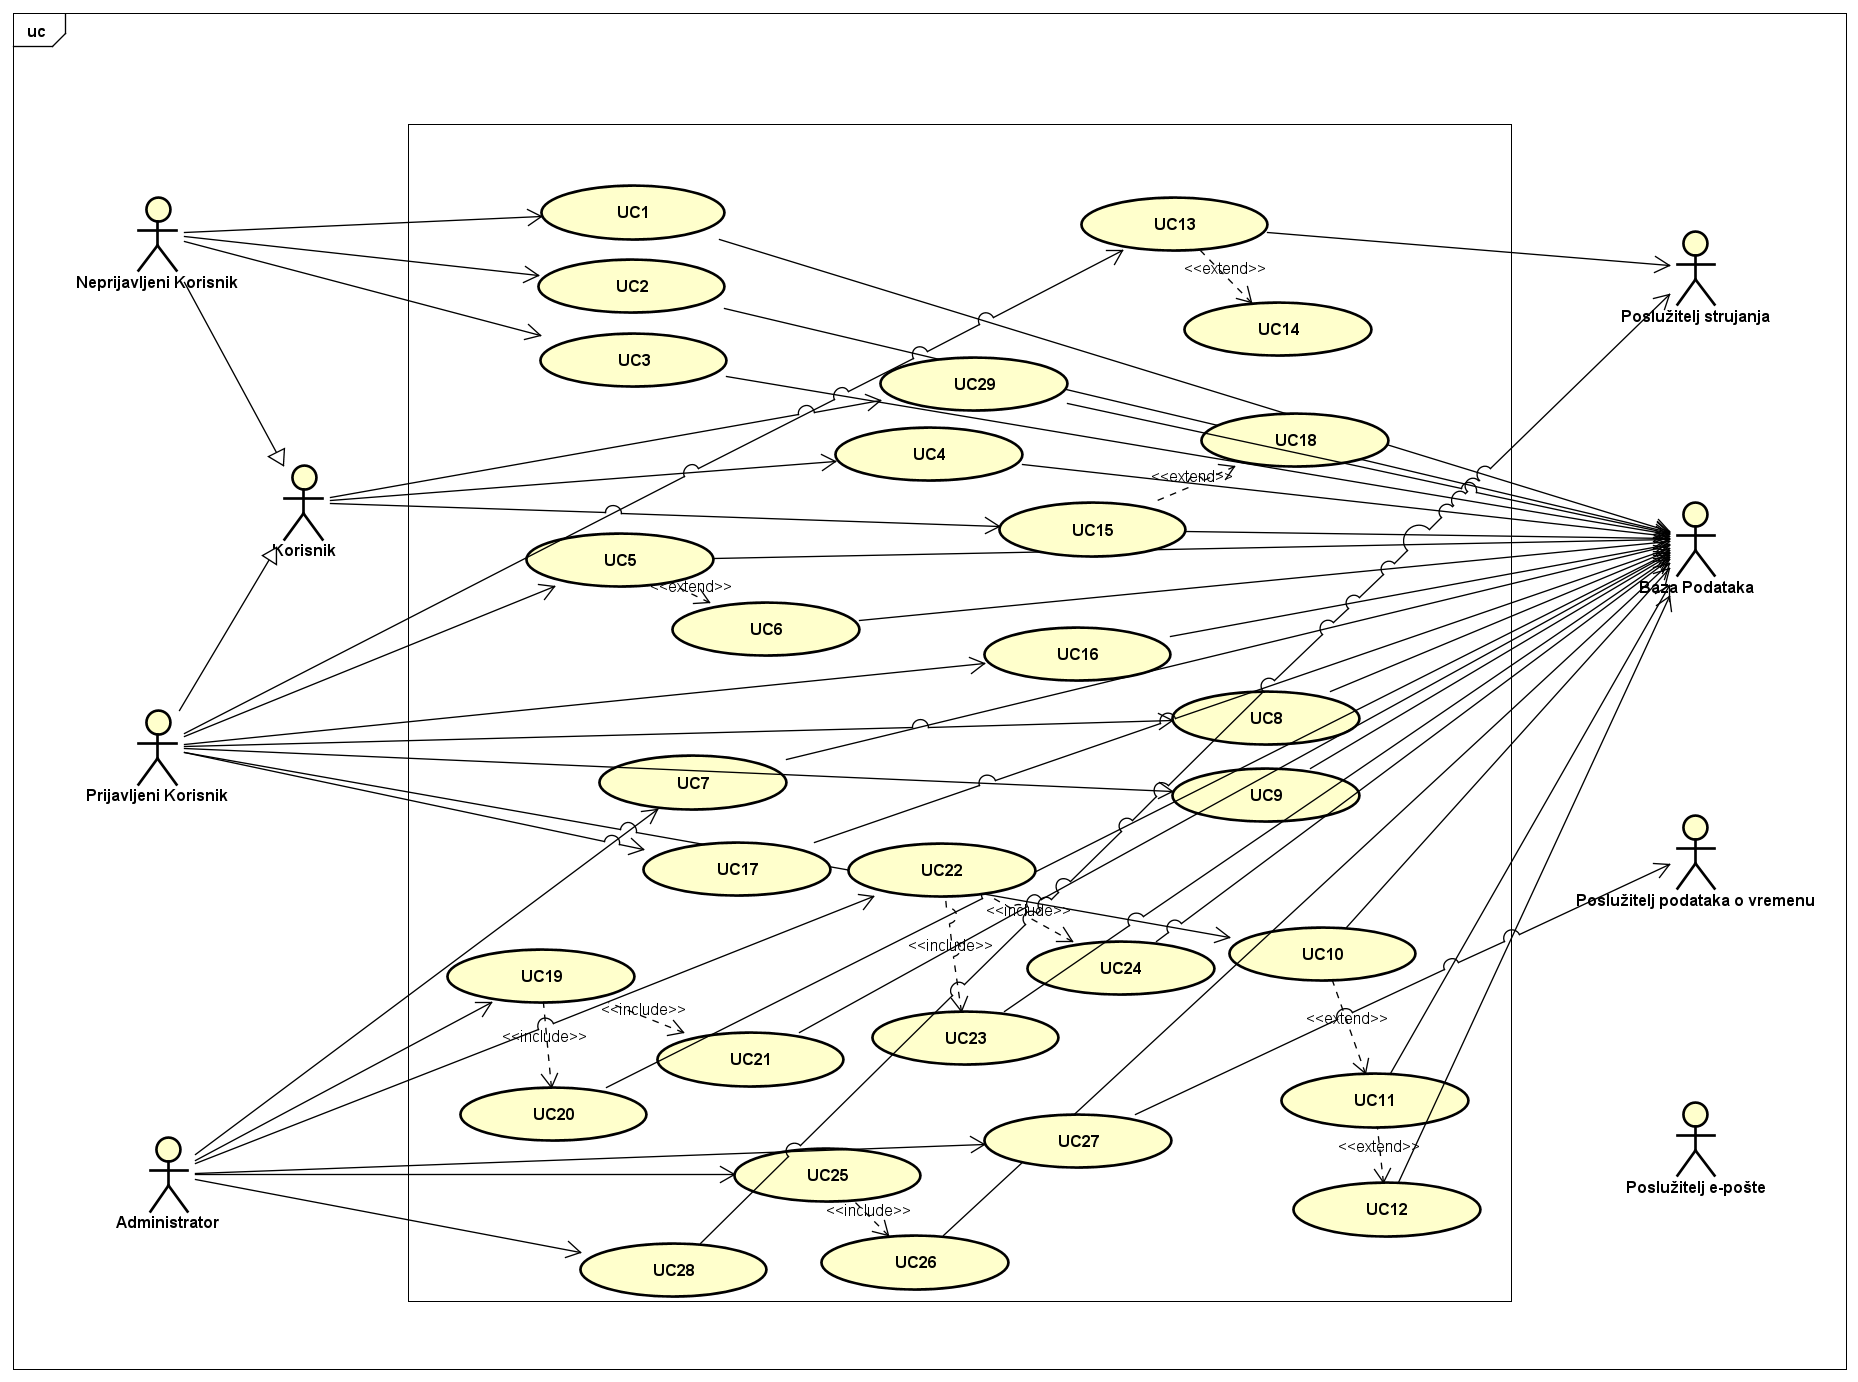
\includegraphics[width=\linewidth]{UseCaseDiagram.png}
						\caption{Početni dijagram obrazaca uporabe}
					\end{figure}
				\eject		
				
			\subsection{Sekvencijski dijagrami}
				
				\textbf{\textit{dio 1. revizije}}\\
				
				\textit{Nacrtati sekvencijske dijagrame koji modeliraju najvažnije dijelove sustava (max. 4 dijagrama). Ukoliko postoji nedoumica oko odabira, razjasniti s asistentom. Uz svaki dijagram napisati detaljni opis dijagrama.}
				\eject
	
		\section{Ostali zahtjevi}
		
			\textbf{\textit{dio 1. revizije}}\\
		 
			 \textit{Nefunkcionalni zahtjevi i zahtjevi domene primjene dopunjuju funkcionalne zahtjeve. Oni opisuju \textbf{kako se sustav treba ponašati} i koja \textbf{ograničenja} treba poštivati (performanse, korisničko iskustvo, pouzdanost, standardi kvalitete, sigurnost...). Primjeri takvih zahtjeva u Vašem projektu mogu biti: podržani jezici korisničkog sučelja, vrijeme odziva, najveći mogući podržani broj korisnika, podržane web/mobilne platforme, razina zaštite (protokoli komunikacije, kriptiranje...)... Svaki takav zahtjev potrebno je navesti u jednoj ili dvije rečenice.}
			 \begin{itemize}
			 	\item Maksimalni broj glasovanja po osobi je 1
			 	\item Glasovanje je moguće samo tijekom određenog vremenskog razdoblja koje je određeno danima i vremenom održavanja konferencije
			 \end{itemize}
			 
			 
			 
	
		\chapter{Arhitektura i dizajn sustava}		
Arhitektura je podijeljena u tri podsustava:

\begin{itemize}
	\item Web poslužitelj
	\item Web aplikacija
	\item Baza podataka
\end{itemize}

\indent Internetski preglednik služi za pregled web-stranica i njihovog višemedijskog sadržaja, a one komuniciraju s poslužiteljima slanjem zahtjeva i primanjem odgovora. Preglednik ima sposobnost interpretacije koda kojim je pisana stranica u ljudski čitljiv oblik.
\newline
\indent Web poslužitelj je posrednik između korisnika i aplikacije, te služi kao osnova rada aplikacije. Komunikacija se ostvaruje korisničkim HTTP (engl. \textit{Hyper Text Transfer Protocol}) zahtjevima koji obično u zaglavlju imaju definiranu GET ili POST metodu za dohvaćanje odnosno predaju podataka. Poslužitelj na njih odgovara dostavom traženog sadržaja.
\newline
\indent Web aplikacija po nalogu poslužitelja pristupa ili mijenja podatke iz baze podataka i vraća HTML dokument koji se potom prikazuje korisniku u sučelju preglednika. Arhitektura sustava će se temeljiti na stilističkoj varijaciji arhitekture zasnovane na događajima (engl. \textit{event based architecture}) - MVC obrazcu. Spring - radni okvir korišten za razvoj pozadinskog dijela aplikacije, podržava MVC (Model-View-Controller) obrazac, te kao takav ima gotove predloške koji nam olakšavaju razvoj web aplikacije.
\newline

\clearpage
\indent MVC obrazac omogućuje odvojen razvoj navedenih slojeva aplikacije što znatno olakšava ispitivanje, razvijanje i dodavanje novih svojstava u sustav.
\newline
Dijelovi MVC obrazca su:
\begin{itemize}
	\item Model(\textit{Model}) - rješava problem interakcije korisnika s bazom podataka, predstavlja bazu i služi za komunikaciju upravljača s bazom, te je na taj način zadužen za logiku vezanu za podatke i njihov prijenos
	\item Prikaz(\textit{View}) - prikaz podataka i njihovih reprezentacija na korisničkom sučelju
	\item Upravljač(\textit{Controller}) - povezuje komponente modela i prikaza i služi kao posrednik između tih komponenata i korisnika, a sam nije zadužen za obradu podataka, međudjeluje s modelom kako bi dohvatio podatke i s prikazom kako bi ih prikazao korisniku
\end{itemize}

\begin{figure} [hbt!]
	
\includegraphics[width=\linewidth]{Slike/ArhitekturaSustava}
	\caption{Reprezentacija arhitekture sustava}
\end{figure}

		\clearpage

		\section{Baza podataka}
			
		Za potrebe našeg sustava koristit ćemo relacijsku bazu podataka koja svojom strukturom olakšava modeliranje stvarnog svijeta. Gradivna jedinka baze je relacija, odnosno tablica koja je definirana svojim imenom i skupom atributa. Zadaća baze podataka je brza i jednostavna pohrana, izmjena i dohvat podataka za daljnju obradu.
		Baza podataka ove aplikacije sastoji se od sljedećih entiteta: 
		
		\begin{itemize}
			\item Konferencija
			\item Korisnik
			\item Poster
			\item Pokrovitelj
			\item Pokrovitelj-Konferencije
			\item Fotografija
		\end{itemize}
		
		\clearpage
		
		\subsection{Opis tablica}
	
	\noindent\textbf{Konferencija }
	
	Ovaj entitet sadržava sve važne informacije o stručnoj konferenciji. Sadrži atribute: identifikator konferencije, ime konferencije, datum i vrijeme početka konferencije, datum i vrijeme završetka konferencije, mjesto održavanja konferencije, adresu održavanja konferencije, poštanski broj mjesta, generičko korisničko ime i pripadajuću lozinku koja se koristi za pristup konferenciji, poveznicu na video prijenos konferencije i oznaku o trajanju glasovanja. Ovaj entitet u vezi je \textit{jedan na više} s entitetom Korisnik preko identifikatora konferencije, u vezi \textit{jedan na više} s entitetom Poster preko identifikatora konferencije, u vezi \textit{jedan na više} s entitetom Fotografija preko identifikatora konferencije i u vezi \textit{više na više} s entitetom Pokrovitelj preko identifikatora konferencije. 
	
	\begin{longtblr}[
		label=none,
		entry=none
		]{
			width = \textwidth,
			colspec={|X[6,l]|X[6, l]|X[20, l]|}, 
			rowhead = 1,
		} %definicija širine tablice, širine stupaca, poravnanje i broja redaka naslova tablice
		\hline \SetCell[c=3]{c}{\textbf{Konferencija}}	 \\ \hline[3pt]
		\SetCell{LightGreen}id\_konferencija & INT	&  	jedinstveni brojčani identifikator konferencije  	\\ \hline
		ime\_ konferencija	& VARCHAR &   jedinstveno ime konferencije	\\ \hline 
		datum\_vrijeme \_pocetka & TIMESTAMP & datum i vrijeme početka konferencije  \\ \hline
		datum\_vrijeme \_zavrsetka & TIMESTAMP & datum i vrijeme završetka konferencije \\ \hline
		mjesto	& VARCHAR & ime mjesta u kojem se održava konferencija \\ \hline 
		adresa & VARCHAR & adresa održavanja konferencije \\ \hline
		zip\_code & VARCHAR & poštanski broj mjesta održavanja konferencije \\ \hline
		generic\_ username	& VARCHAR & generičko korisničko ime koje koriste svi posjetitelji konferencije prije izrade vlastitog korisničkog računa  \\ \hline 
		generic\_ password & VARCHAR & hash lozinka generičkog korisničkog računa \\ \hline
		video\_url & VARCHAR & poveznica na video prijenos konferencije \\ \hline
		voting\_ reminder\_sent & BOOLEAN & oznaka pomoću koje aplikacija svakih 24 sata provjerava traje li glasanje za zadanu konferenciju \\ \hline
	\end{longtblr}
	
	\clearpage
	
	\noindent\textbf{Korisnik }
	
	Ovaj entitet sadržava sve važne informacije o korisniku aplikacije. Sadrži atribute: identifikator korisnika, e-mail adresu korisnika, lozinku, ime, prezime, oznaku ima li korisnik ovlasti administratora, oznaku radi li se o generičkom računu, oznaku je li korisnik glasao i identifikator konferencije na kojoj korisnik sudjeluje.  Ovaj entitet je u vezi \textit{više na jedan} s entitetom Konferencija preko identifikatora konferencije. 
	
	\begin{longtblr}[
		label=none,
		entry=none
		]{
			width = \textwidth,
			colspec={|X[6,l]|X[6, l]|X[20, l]|}, 
			rowhead = 1,
		} %definicija širine tablice, širine stupaca, poravnanje i broja redaka naslova tablice
		\hline \SetCell[c=3]{c}{\textbf{Korisnik}}	 \\ \hline[3pt]
		\SetCell{LightGreen}id\_korisnik & INT &  jedinstveni brojčani identifikator korisnika	\\ \hline
		email & VARCHAR	&  e-mail adresa kojom korisnik izrađuje korisnički račun 	\\ \hline
		lozinka	& VARCHAR & hash lozinka korisničkog računa  	\\ \hline 
		ime & VARCHAR & ime korisnika  \\ \hline 
		prezime & VARCHAR	& prezime korisnika 		\\ \hline 
		admin & BOOLEAN &  oznaka ima li ovlasti administratora		\\ \hline 
		visitor & BOOLEAN &  oznaka radi li se o generičkom računu (TRUE), kada posjetitelj napravi vlastiti korisnički račun vrijednost varijable postaje FALSE	\\ \hline 
		voted & BOOLEAN & oznaka je li korisnik glasao \\ \hline
		\SetCell{LightBlue} id\_konferencija	& INT & jedinstveni identifikator konferencije na kojoj korisnik sudjeluje (konferencija.id\_konferencija)  	\\ \hline 
	\end{longtblr}
	
	\clearpage
	
	\noindent \textbf{Poster }
	
	Ovaj entitet sadržava sve važne informacije o radu prikazanom odgovarajućim posterom/prezentacijom. Sadrži atribute: identifikator postera, ime postera, datoteku postera, broj glasova za poster, ime i prezime autora, e-mail adresu kojom je autor poslao poster i identifikator konferencije na kojoj se rad izlaže. Ovaj entitet je u vezi \textit{više na jedan} s entitetom Konferencija preko identifikatora konferencije.
	
	
	\begin{longtblr}[
		label=none,
		entry=none
		]{
			width = \textwidth,
			colspec={|X[6,l]|X[6, l]|X[20, l]|}, 
			rowhead = 1,
		} %definicija širine tablice, širine stupaca, poravnanje i broja redaka naslova tablice
		\hline \SetCell[c=3]{c}{\textbf{Poster}}	 \\ \hline[3pt]
		\SetCell{LightGreen}id\_poster & INT &  jedinstveni brojčani identifikator postera	\\ \hline
		ime\_poster & VARCHAR	&  ime postera\\ \hline
		file\_path & LONGBLOB & PDF datoteka postera ili prezentacije  \\ \hline 
		br\_glasova & INT & broj glasova za određeni poster \\ \hline 
		ime\_autor & VARCHAR & ime autora \\ \hline
		prezime\_autor & VARCHAR & prezime autora \\ \hline
		poster\_email & VARCHAR & e-mail adresa autora \\ \hline
		\SetCell{LightBlue} id\_konferencija	& INT & jedinstveni brojčani identifikator konferencije kojoj poster pripada (konferencija.id\_konferencija)  	\\ \hline 
	\end{longtblr}
	
	\clearpage
	
	\noindent \textbf{Pokrovitelj }
	
	Ovaj entitet sadržava sve važne informacije o pokrovitelju. Sadrži atribute: ime pokrovitelja, promotivne materijale i poveznicu na stranicu pokrovitelja. Ovaj entitet je u vezi \textit{više na više} s entitetom Konferencija.
	
	
	\begin{longtblr}[
		label=none,
		entry=none
		]{
			width = \textwidth,
			colspec={|X[6,l]|X[6, l]|X[20, l]|}, 
			rowhead = 1,
		} %definicija širine tablice, širine stupaca, poravnanje i broja redaka naslova tablice
		\hline \SetCell[c=3]{c}{\textbf{Pokrovitelj}}	 \\ \hline[3pt]
		\SetCell{LightGreen}ime\_ pokrovitelja & VARCHAR & jedinstveni identifikator pokrovitelja  	\\ \hline
		promotivni\_ materijal & LONGBLOB & datoteka, promotivni materijal je logotip pokrovitelja   \\ \hline 
		url\_promo & VARCHAR & poveznica na stranicu pokrovitelja \\ \hline 
	\end{longtblr}
	
	\noindent \textbf{Pokrovitelj-Konferencije }
	
	Ovaj entitet nastaje zbog \textit{više na više} veze između entiteta Konferencija i Pokrovitelj. Sadržava sve informacije o odnosu konferencije i pokrovitelja odnosno kojoj konferenciji pokrovitelj pripada. 
	
	
	\begin{longtblr}[
		label=none,
		entry=none
		]{
			width = \textwidth,
			colspec={|X[6,l]|X[6, l]|X[20, l]|}, 
			rowhead = 1,
		} %definicija širine tablice, širine stupaca, poravnanje i broja redaka naslova tablice
		\hline \SetCell[c=3]{c}{\textbf{Pokrovitelj-Konferencije}}	 \\ \hline[3pt]
		\SetCell{LightBlue} ime\_
		pokrovitelja	& VARCHAR & jedinstveni identifikator pokrovitelja (pokrovitelj.imePokrovitelja)     	\\ \hline
		\SetCell{LightBlue}id\_konferencija	& INT & jedinstveni brojčani identifikator konferencije (konferencija.id\_konferencija)  	\\ \hline 
		
	\end{longtblr}
	
	
	\noindent \textbf{Fotografija }
	
	Ovaj entitet sadržava sve informacije o fotografijama s konferencije. Sadrži atribute: identifikator fotografije, sliku fotografije i identifikator konferencije kojoj fotografija pripada. Ovaj entitet u vezi je \textit{više na jedan} s entitetom Konferencija. 
	
	
	\begin{longtblr}[
		label=none,
		entry=none
		]{
			width = \textwidth,
			colspec={|X[6,l]|X[6, l]|X[20, l]|}, 
			rowhead = 1,
		} %definicija širine tablice, širine stupaca, poravnanje i broja redaka naslova tablice
		\hline \SetCell[c=3]{c}{\textbf{Fotografije}}	 \\ \hline[3pt]
		\SetCell{LightGreen}id\_fotografija & INT & jedinstveni brojčani identifikator fotografije   	\\ \hline
		file\_path	& LONGBLOB &  fotografije	\\ \hline 
		\SetCell{LightBlue} id\_konferencija	& INT & jedinstveni brojčani identifikator konferencije kojoj fotografija pripada (konferencija.id\_konferencija)	\\ \hline 
	\end{longtblr}
	
	\clearpage
			
			\subsection{Dijagram baze podataka}
				
					\begin{figure} [h]
						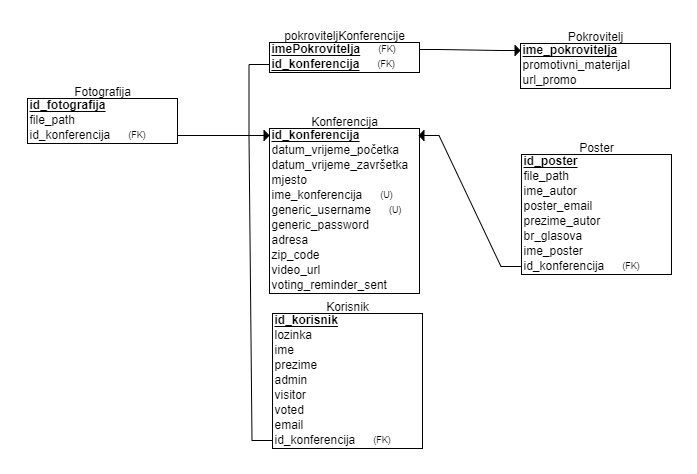
\includegraphics[width=\linewidth]{Slike/ERDijagram}
						\caption{E-R dijagram baze podataka}
					\end{figure}
			
			\eject
			
			
		\section{Dijagram razreda}
			
			\indent Slike 4.3, 4.4 i 4.5 prikazuju dijagrame razreda pozadinskog dijela MVC arhitekture. Slike 4.3 i 4.4 prikazuju upravljačke razrede, te DAO (\textit{Data Access Object} razrede. 
			
			Dijagrami su zbog preglednosti podijeljeni po slojevima, odnosno na pojedinom dijagramu prikazane su samo ovisnosti između razreda istog MVC sloja, a prema nazivima samih razreda može se logički zaključiti koji su razredi različitih slojeva funkcionalno povezani.
			
			Razredi dijagrama na slici 4.5 preslikavaju entitete i atribute baze podataka. Razred Korisnik predstavlja općeniti model korisnika aplikacije koji može biti posjetitelj konferencije ili administrator. Može se registrirati u sustav unoseći osnove informacije. Razred Konferencija predstavlja skup podataka koji su potrebni za registraciju konferencije i koji se prikazuju korisnicima. Razred Poster predstavlja skup podataka koji su potrebni za dodavanje postera i koji se prikazuju korisnicima. Razred Fotografija predstavlja skup podataka vezan uz pojedinačnu fotografiju konferencije. Razred Pokrovitelj predstavlja pokrovitelja konferencije.
			
			\begin{figure} [hbt!]
				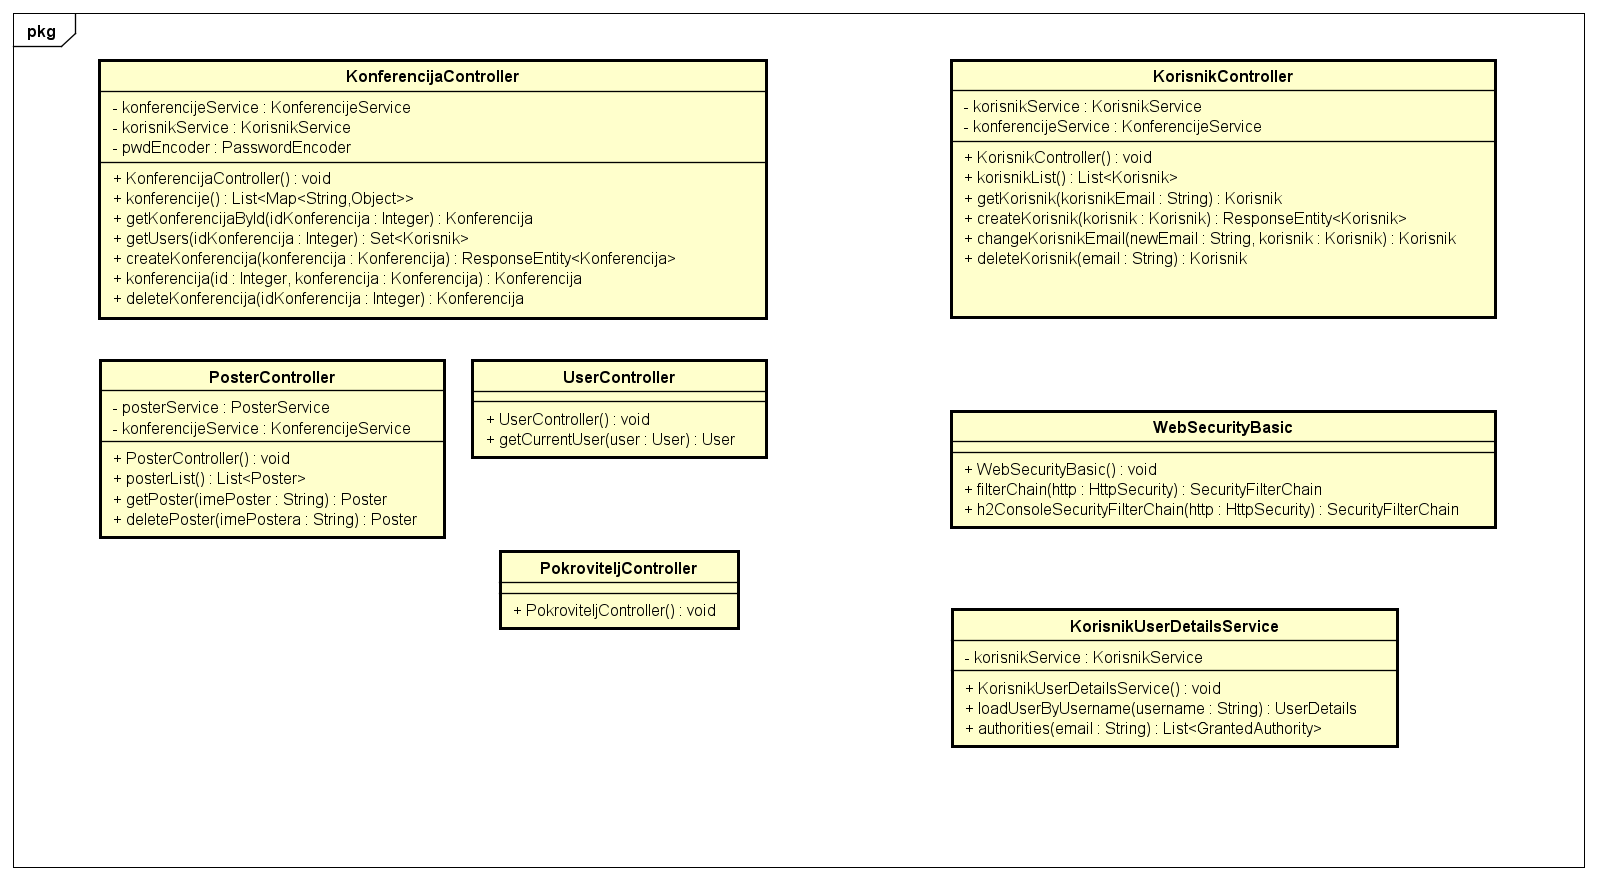
\includegraphics[width=\linewidth]{Slike/ClassDiagramControllerPremaKodu}
				\caption{Dijagram razreda - Upravljači}
			\end{figure}
			
			\begin{figure} [hbt!]
				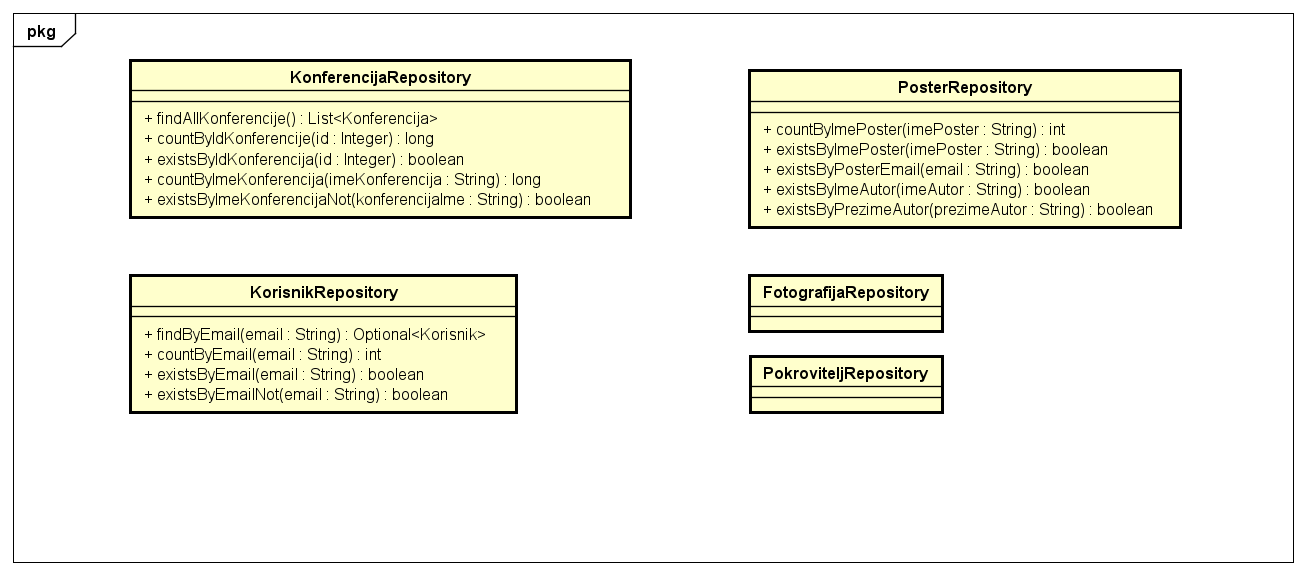
\includegraphics[width=\linewidth]{Slike/ClassDiagramRepositoryPremaKodu}
				\caption{Dijagram razreda - DAO}
			\end{figure}
			
			\begin{figure} [hbt!]
				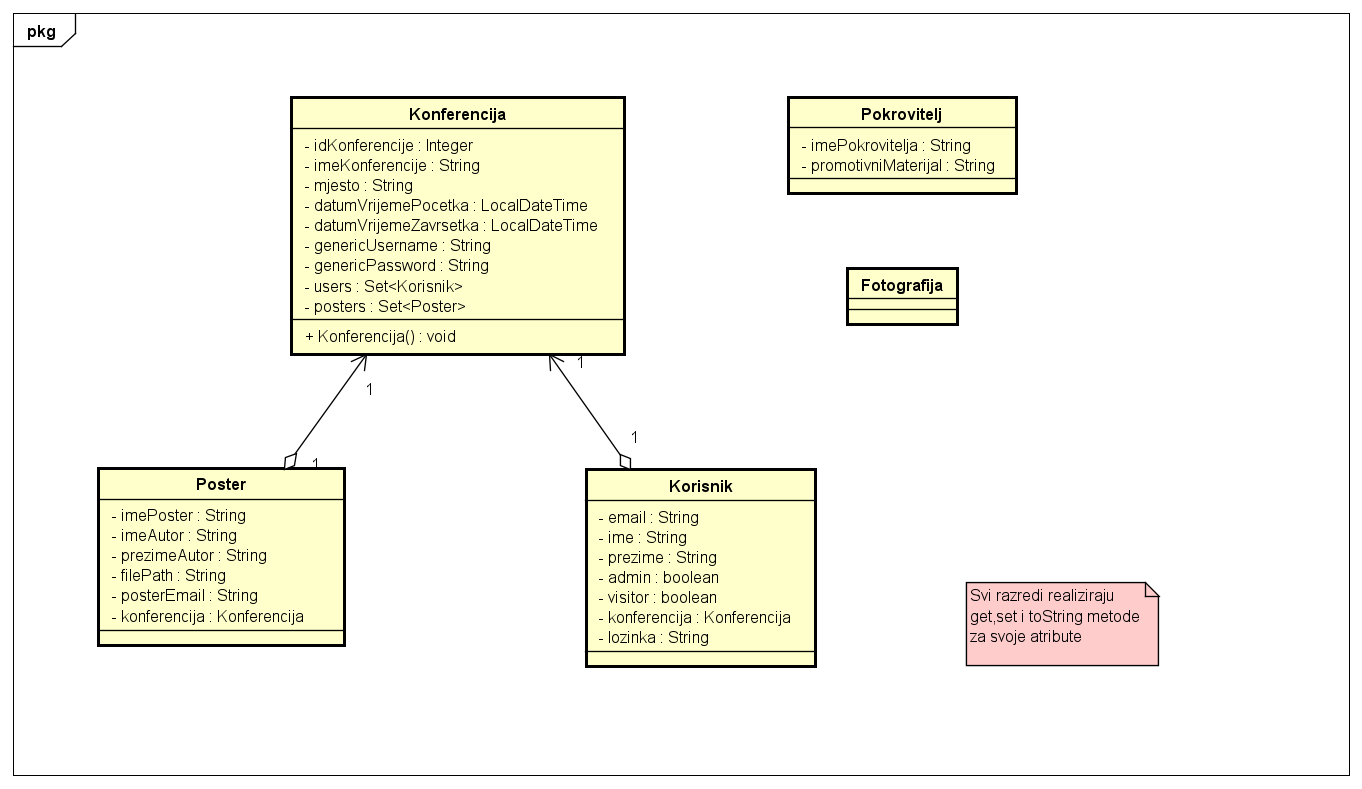
\includegraphics[width=\linewidth]{Slike/ClassDiagramModelPremaKodu}
				\caption{Dijagram razreda - Modeli}
			\end{figure}
			
			\clearpage
			 
			\textbf{\textit{dio 2. revizije}}\\			
			
			\textit{Prilikom druge predaje projekta dijagram razreda i opisi moraju odgovarati stvarnom stanju implementacije}
			
			
			
			\eject
		
		\section{Dijagram stanja}
			
			
			\textbf{\textit{dio 2. revizije}}\\
			
			\textit{Potrebno je priložiti dijagram stanja i opisati ga. Dovoljan je jedan dijagram stanja koji prikazuje \textbf{značajan dio funkcionalnosti} sustava. Na primjer, stanja korisničkog sučelja i tijek korištenja neke ključne funkcionalnosti jesu značajan dio sustava, a registracija i prijava nisu. }
			
			\indent Dijagram stanja opisuje ponašanje sustava koristeći konačan broj apstraktnih diskretnih stanja u kojima se on može nalaziti i načine na koje se može prijeći iz jednog u drugo stanje, odnosno korisničke akcije koje potiču te prijelaze. Na slici 4.6 je prikazan dijagram stanja za registriranog korisnika koji je prije same registracije pristupio konferenciji pomoću generičke lozinke. Registriranom korisniku omogućen je pregled samo onih konferencija kojima je pristupio. Nakon uspješnog pristupa konferenciji, korisniku se prikazuje početna stranica konferencije na kojoj može pregledati vrijeme i mjesto događaja, vremensku prognozu za idućih 48 sati na toj lokaciji, te video prijenos konferencije, kao i popis pokrovitelja konferencije. Navigacijska traka korisniku omogućava pristup posterima, fotografijama, te pokroviteljima konferencije. Klikom na "Posteri" prikazuje mu se galerija postera gdje ima mogućnost glasanja za poster po izboru unutar zadanog vremenskog ograničenja. Klikom na "Fotografije" otvara se galerija fotografija, odakle se odabrane fotografije mogu preuzeti na računalo. Klikom na "Pokrovitelji", korisniku se prikazuju pokrovitelji konferencije. Klikom na logo određenog pokrovitelja otvoriti će se službena stranica pokrovitelja koja se nalazi izvan aplikacije. Nakon završetka glasovanja korisnik će imati pristup rezultatima klikom na "Rezultati".
			
			\begin{figure} [hbt!]
				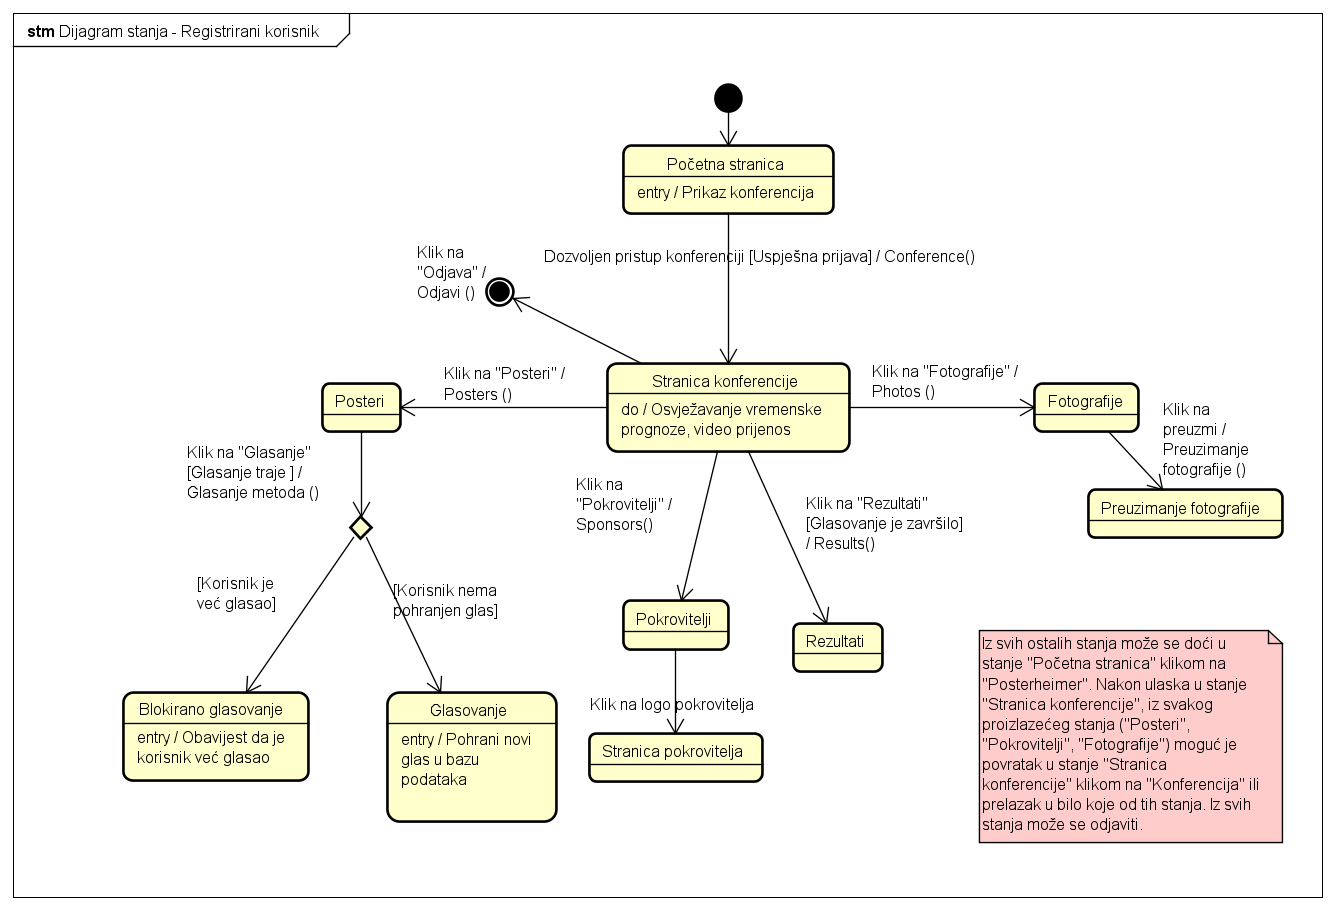
\includegraphics[width=\linewidth]{Slike/StateMachineDiagram}
				\caption{Dijagram stanja}
			\end{figure}
			
			
			\eject 
		
		\section{Dijagram aktivnosti}
			
			\textbf{\textit{dio 2. revizije}}\\
			
			 \textit{Potrebno je priložiti dijagram aktivnosti s pripadajućim opisom. Dijagram aktivnosti treba prikazivati značajan dio sustava.}
			 
			 \indent Dijagram aktivnosti opisuje ponašanje funkcionalnog dijela sustava, te interakciju više fizički ili programski odvojenih dijelova sustava, a posebno je pogodan za prikaz njihove sinkronizacije i konkurentnog djelovanja. Dijagram aktivnosti na slici 4.7 prikazuje tok podataka postupka glasovanja za poster. Korisnik pristupa aplikaciji i odabire konferenciju na kojoj sudjeluje. Klikom na opciju "Posteri" korisniku će se prikazati galerija postera. Korisnik odabire jedan poster te za njega glasa.    
			 
			 \begin{figure}
			 	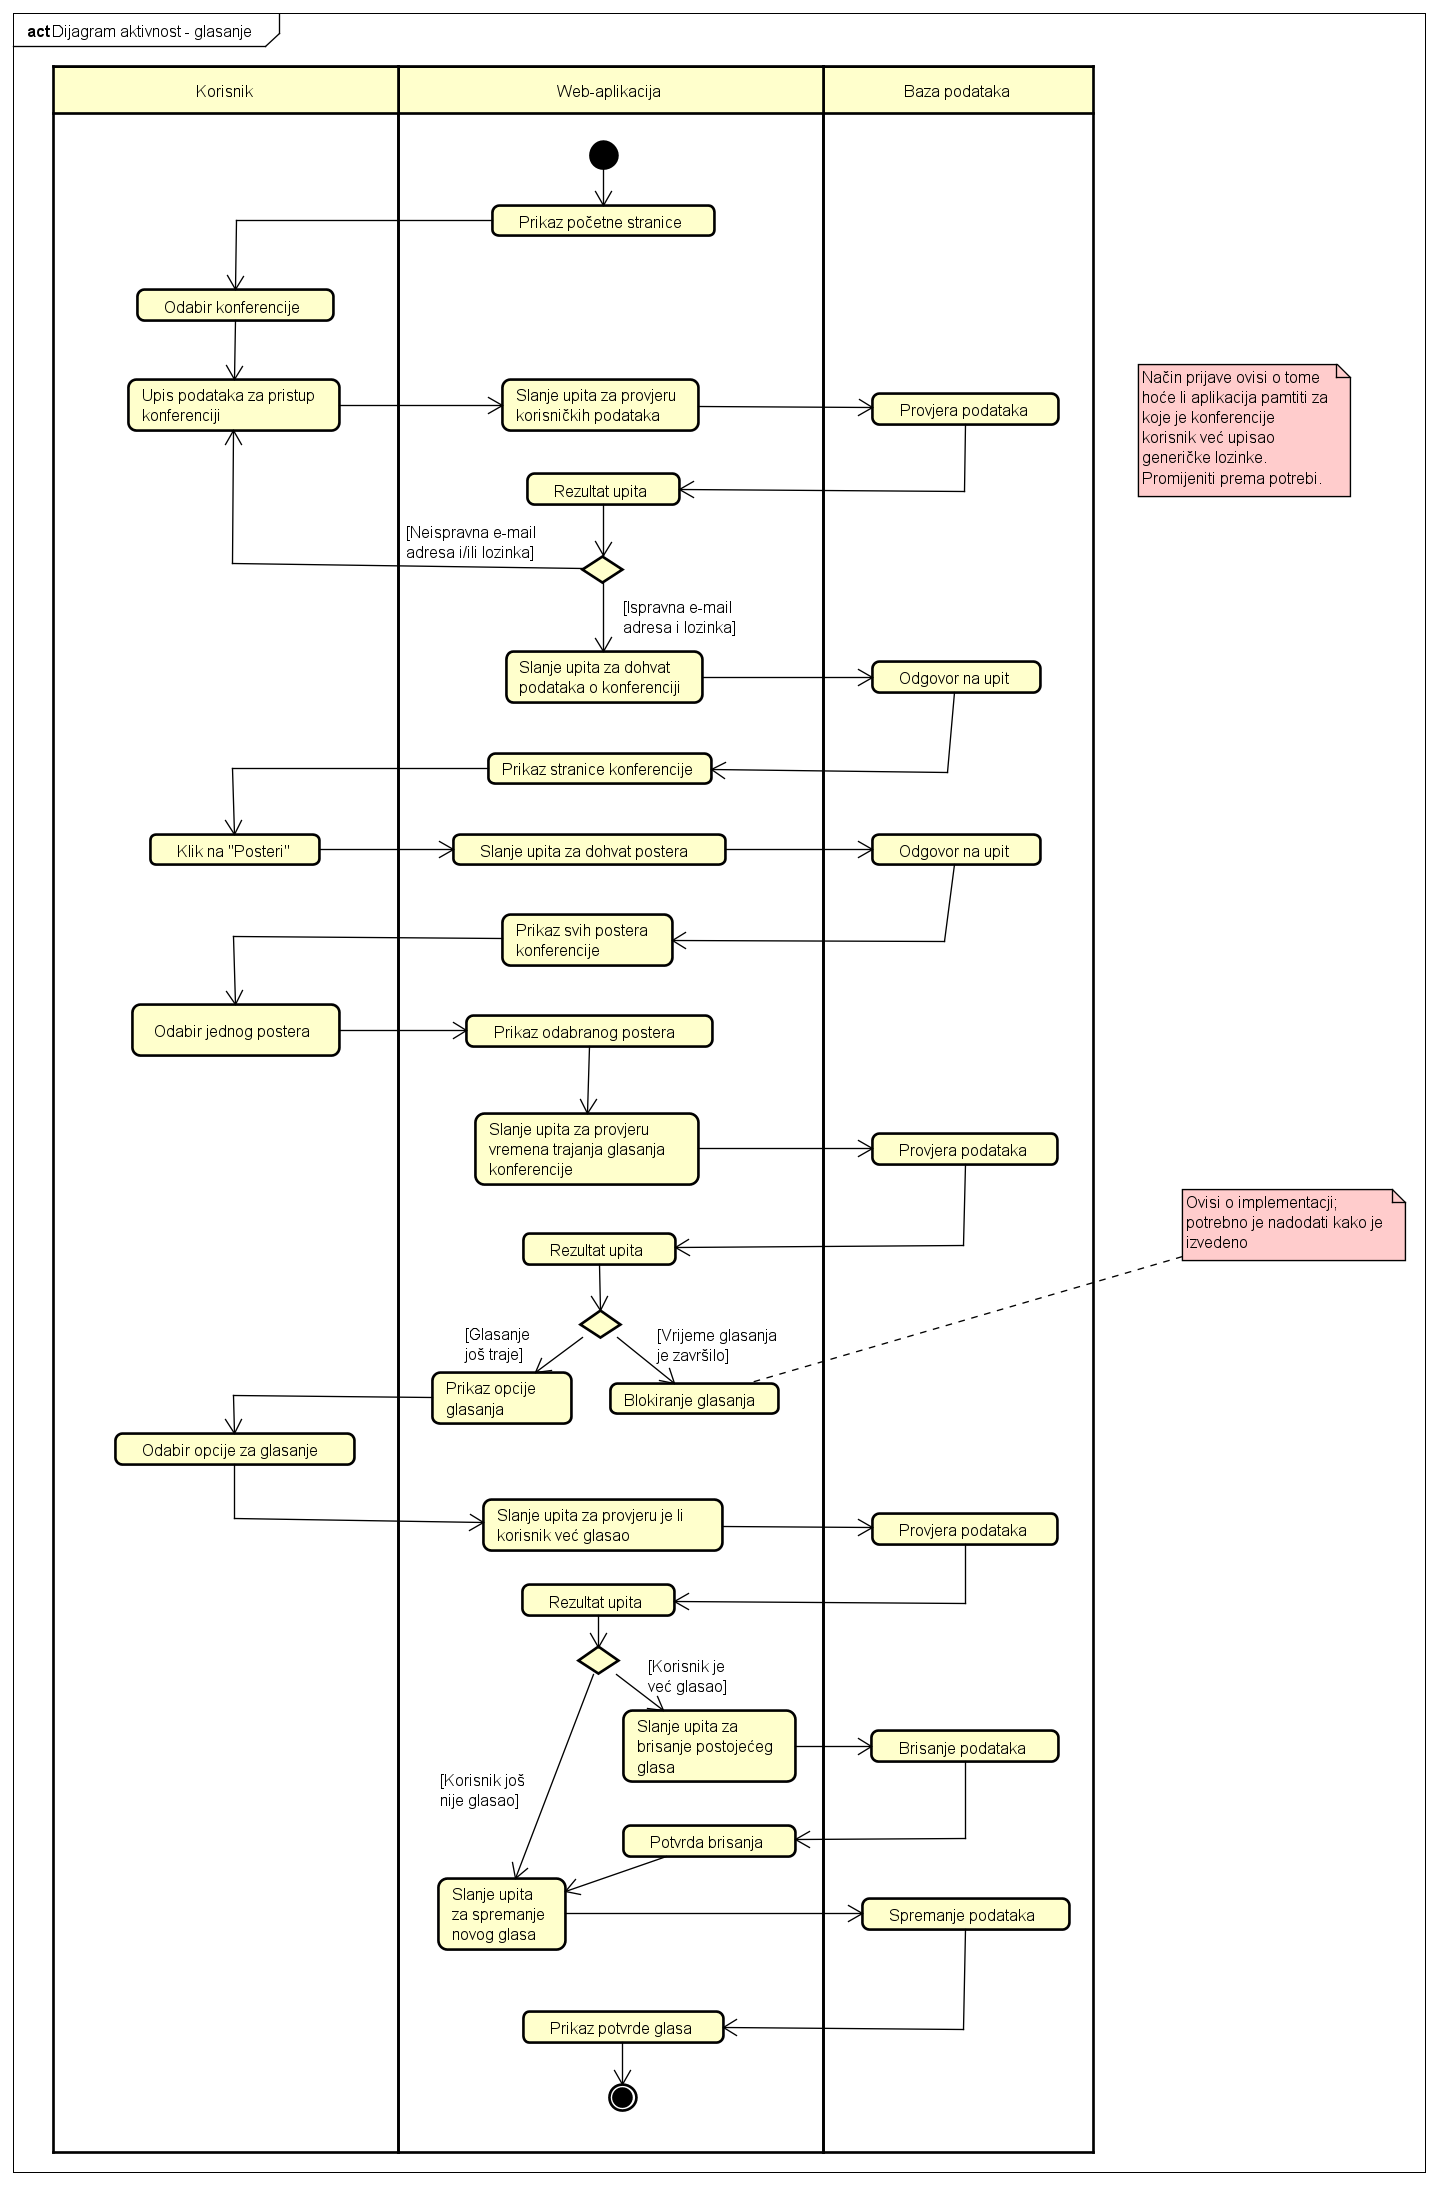
\includegraphics[width=\linewidth]{Slike/ActivityDiagram}
			 	\caption{Dijagram aktivnosti - Glasovanje}
			 \end{figure}
			
			\eject
		\section{Dijagram komponenti}
		
			\textbf{\textit{dio 2. revizije}}\\
		
			 \textit{Potrebno je priložiti dijagram komponenti s pripadajućim opisom. Dijagram komponenti treba prikazivati strukturu cijele aplikacije.}
			 
			 \indent Dijagram komponenti prikazan na slici 4.8 vizualizira organizaciju programskih komponenti i cjelina, te njihovu međuovisnost i međusobnu interakciju preko nuđenih i traženih sučelja. Sustavu se pristupa preko dva različita sučelja. Preko sučelja za dohvat HTML, CSS i JSX datoteka poslužuju se datoteke koje pripadaju prednjem \textit{engl. frontend} dijelu aplikacije. AppRouter je komponenta koja na upit s url određuje koja datoteka će se poslužiti na sučelje. Prednji \textit{engl. frontend} dio sastoji se od niza JavaScript XML datoteka koje su raspoređene u logičke cjeline nazvane po dijelu aplikacije za koji se koriste. Sve JavaScript XML datoteke ovise o React biblioteci iz koje dohvaćaju gotove komponente. Preko sučelja za dohvat JSON podataka pristupa se REST API komponenti. REST API poslužuje podatke koji pripadaju \textit{backend} dijelu aplikacije. Repository je zadužen za dohvaćanje tablica iz baze podataka pomoću SQL upita. Podaci koji su pristigli iz baze se šalju dalje MVC arhitekturi u obliku DTO \textit{(Data transfer object)}. React-view komponenta preko dostupnih sučelja komunicira sa Posterheimer aplikacijom te ovisno o korisnikovim akcijama osvježava prikaz i dohvaća nove podatke ili datoteke.
			 
			 \begin{figure}
			 	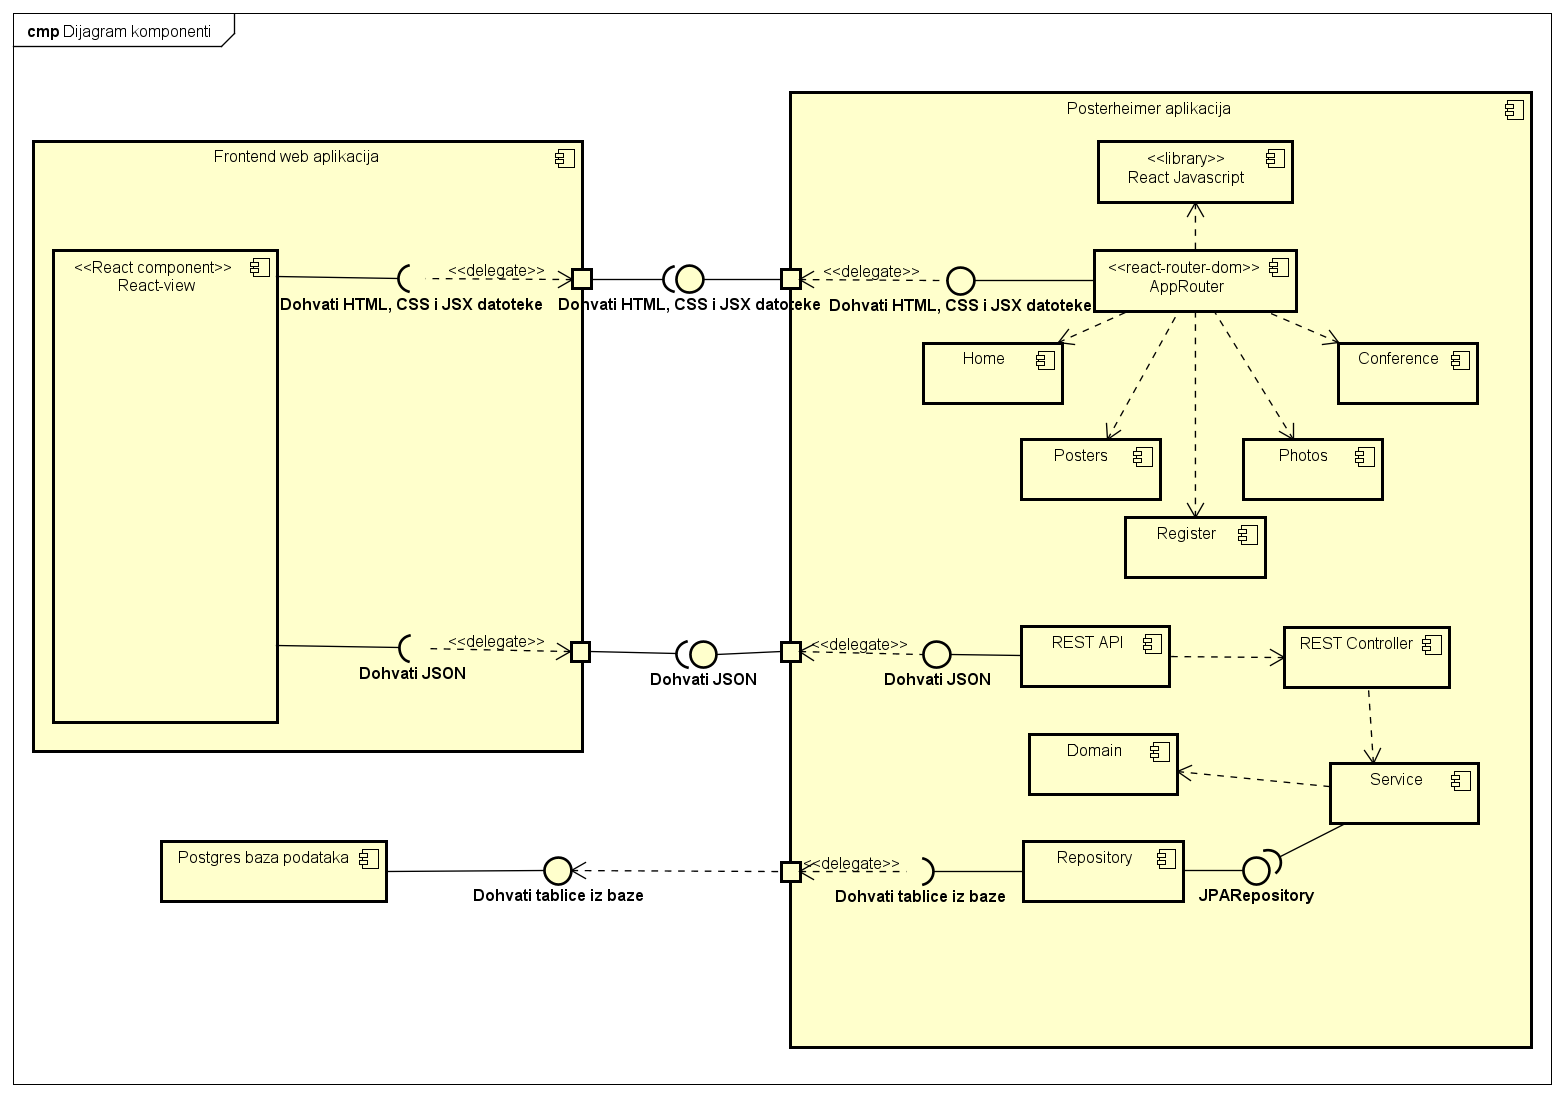
\includegraphics[width=\linewidth]{Slike/ComponentDiagram}
			 	\caption{Dijagram komponenti}
			 \end{figure}
		\chapter{Implementacija i korisničko sučelje}
		
		
		\section{Korištene tehnologije i alati}
		
			\textbf{\textit{dio 2. revizije}}
			
			 \textit{Detaljno navesti sve tehnologije i alate koji su primijenjeni pri izradi dokumentacije i aplikacije. Ukratko ih opisati, te navesti njihovo značenje i mjesto primjene. Za svaki navedeni alat i tehnologiju je potrebno \textbf{navesti internet poveznicu} gdje se mogu preuzeti ili više saznati o njima}.
			
			\indent Pri izradi dokumentacije korišten je \textbf{LaTeX}\footnote{https://www.latex-project.org} - označni jezik korišten za uređivanje tekstualnih dokumenata najčešće znanstvene publikacije. Dokument je sastavljen u programu \textbf{TeXstudio}\footnote{https://www.texstudio.org} - uređivaču teksta prilagođen LaTeX-u. UML dijagrami nacrtani su uz pomoć alata \textbf{Astah UML}\footnote{https://astah.net/products/astah-uml}. Dijagrami koji nisu UML tipa nacrtani su u uređivaču \textbf{MS Word}\footnote{https://www.microsoft.com/en/microsoft-365/word}
			
			Udaljeni repozitorij projekta dostupan je na platformi \textbf{GitHub}\footnote{https://github.com}, korištenoj za pohranu svih datoteka potrebnih za rad na projektu.
			
			Za izradu pozadinskog dijela aplikacije korišten je objektno orijentirani programski jezik \textbf{Java}\footnote{https://www.java.com/en} i radni okvir \textbf{Spring Boot}\footnote{https://spring.io/projects/spring-boot} - specijalizacija radnog okvira Spring, s ciljem jednostavnijeg i bržeg oblikovanja web aplikacije. Kao razvojno okruženje korišten je \textbf{IntelliJ IDEA}\footnote{https://www.jetbrains.com/idea}. Tijekom izrade, pozadinski dio aplikacije testiran je pomoću platforme za testiranje API-ja \textbf{Postman}\footnote{https://www.postman.com}.
			
			Za izradu prednjeg dijela aplikacije korišten je \textbf{React}\footnote{https://react.dev} i JavaScript ekstenzija \textbf{JavaScript XML}\footnote{https://legacy.reactjs.org/docs/introducing-jsx.html}. React, također poznat kao React.js ili ReactJS, je biblioteka u JavaScriptu za izgradnju korisničkih sučelja koju održava \textit{Facebook}. \textit{React} se najčešće koristi kao osnova u razvoju mrežnih ili mobilnih aplikacija. Složene aplikacije u \textit{React}-u obično zahtijevaju korištenje dodatnih biblioteka za interakciju s API-jem.
			
			Baza podataka izrađena je u sustavu za upravljanje bazama podataka \textbf{PostgreSQL}\footnote{https://www.postgresql.org}. Za pristup PostgreSQL sustavu baze podataka korišten je \textbf{pgAdmin 4}\footnote{https://www.pgadmin.org} program. Za izradu ER dijagrama baze podataka korišten je \textbf{ERDPlus}\footnote{https://erdplus.com} alat.
			
			Aplikacija i baza podataka su postavljene na udaljene poslužitelje kao usluga aplikacije \textbf{Render}\footnote{https://render.com}, koja nudi besplatnu opciju pri iznajmljivanju sklopovlja, s ograničenim mogućnostima.
			
			Komunikacija između članova tima ostvarena je putem aplikacija s tom svrhom: \textbf{WhatsApp}\footnote{https://www.whatsapp.com} i \textbf{Discord}\footnote{https://discord.com}.
			
			\eject 
		
	
		\section{Ispitivanje programskog rješenja}
			
			\textbf{\textit{dio 2. revizije}}\\
			
			 \textit{U ovom poglavlju je potrebno opisati provedbu ispitivanja implementiranih funkcionalnosti na razini komponenti i na razini cijelog sustava s prikazom odabranih ispitnih slučajeva. Studenti trebaju ispitati temeljnu funkcionalnost i rubne uvjete.}
			 
			
			\subsection{Ispitivanje komponenti}
			\textit{Potrebno je provesti ispitivanje jedinica (engl. unit testing) nad razredima koji implementiraju temeljne funkcionalnosti. Razraditi \textbf{minimalno 6 ispitnih slučajeva} u kojima će se ispitati redovni slučajevi, rubni uvjeti te izazivanje pogreške (engl. exception throwing). Poželjno je stvoriti i ispitni slučaj koji koristi funkcionalnosti koje nisu implementirane. Potrebno je priložiti izvorni kôd svih ispitnih slučajeva te prikaz rezultata izvođenja ispita u razvojnom okruženju (prolaz/pad ispita). }
			
			Ispitivanje komponenti provedeno je pomoću Selenium WebDrivera\footnote{https://www.selenium.dev/documentation/webdriver/} unutar JUnit 4 testova kao podršku za pisanje ispita unutar programskog jezika Java. Ispitivanje je provedeno nad konferencijom naziva "TestKonferencija". U vrijeme izrade dokumentacije, konferencija se nalazila na drugom mjestu na listi dostupnih konferencija. 
			Izrađeno je 7 ispitnih slučajeva. Uspješnost 6 slučajeve te izazivanje pogreške u jednom prikazani su slikom 5.1.
			
			\begin{figure} [hbt!]
				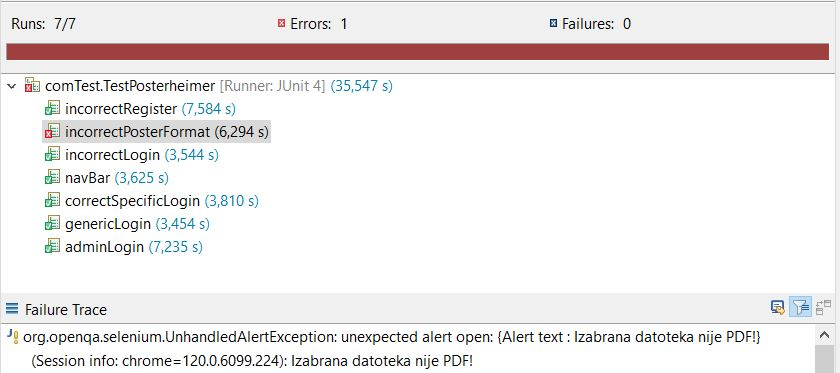
\includegraphics[width=\linewidth]{Slike/testResults}
				\caption{Prikaz uspješnosti ispitnih slučajeva}
			\end{figure}
			
			U \textbf{prvom ispitnom slučaju} provjerena je funkcionalnost gumba za pristup konferenciji pri inicijalnom pristupu pomoću točnog generičkog korisničkog imena (adrese e-pošte predviđenu za generički račun) i odgovarajuće lozinke. Predviđen rezultat je dozvoljen pristup stranici konferencije. Ispitni slučaj je uspješan.
			
			
			\begin{lstlisting}
@Test
public void genericLogin() {
	
	System.setProperty("webdriver.chrome.driver", "src\\test\\java\\chromedriver\\chromedriver.exe");
	WebDriver driver = new ChromeDriver();
	driver.manage().timeouts().implicitlyWait(10, TimeUnit.SECONDS);
	
	driver.get("https://posterheimer.onrender.com/");
	org.openqa.selenium.Dimension target = new  org.openqa.selenium.Dimension(1552, 840);
	driver.manage().window().setSize(target);
	
	driver.findElement(By.xpath("(//button[contains(text(),'Pristupi')])[2]")).click();
	// broj postaviti na mjesto konferencije u listi
	
	driver.findElement(By.id("username")).click();
	driver.findElement(By.id("username")).sendKeys("visitor.test@mail.hr");
	driver.findElement(By.id("password")).click();
	driver.findElement(By.id("password")).sendKeys("Lozinka1");
	driver.findElement(By.cssSelector(".btn-primary")).click();
	
	driver.findElement(By.linkText("Konferencija")).click();
	
	String redirURL = driver.getCurrentUrl();
	boolean comperRes = redirURL.contains("/conference");
	if(comperRes == true) {
		System.out.println("Pristupljeno konferenciji");
	} else {
		System.out.println("Error");
	}
	assertEquals(comperRes, true);
	driver.quit();
}
			\end{lstlisting}
			
			U \textbf{drugom ispitnom slučaju} provjerena je funkcionalnost gumba za pristup konferenciji pomoću jedinstvenog korisničkog računa, te odjava. Potrebno je upisati točnu adresu e-pošte i odgovarajuću lozinku već stvorenog korisničkog računa. Nakon upisa podataka, korisnik dobiva pristup stranici konferencije. Nakon prijave, korisnik se odjavljuje. Predviđen rezultat je povratak na početnu stranicu aplikacije. Ispitni slučaj je uspješan.  

			
			\begin{lstlisting}
@Test
public void correctSpecificLogin() {
	System.setProperty("webdriver.chrome.driver", "src\\test\\java\\chromedriver\\chromedriver.exe");
	WebDriver driver = new ChromeDriver();
	driver.manage().timeouts().implicitlyWait(10, TimeUnit.SECONDS);
	
	driver.get("https://posterheimer.onrender.com/");
	driver.manage().window().setSize(new Dimension(1552, 840));
	driver.findElement(By.cssSelector(".list-group-item:nth-child(4) > .float-end")).click();
	driver.findElement(By.id("username")).click();
	driver.findElement(By.id("username")).sendKeys("register.email@mail.hr");
	driver.findElement(By.id("password")).click();
	driver.findElement(By.id("password")).sendKeys("Lozinka1");
	driver.findElement(By.cssSelector(".btn-primary")).click();
	
	driver.findElement(By.linkText("Konferencija")).click();
	
	String redirURL = driver.getCurrentUrl();
	boolean comperRes = redirURL.contains("/conference");
	if(comperRes == true) {
		System.out.println("Pristupljeno konferenciji");
	} else {
		System.out.println("Error: prijava");
	}
	
	driver.findElement(By.id("user-dropdown")).click();
	driver.findElement(By.cssSelector(".fa-right-from-bracket")).click();
	
	redirURL = driver.getCurrentUrl();
	comperRes = redirURL.equals("https://posterheimer.onrender.com/");
	if(comperRes == true) {
		System.out.println("Ostvarena odjava");
	} else {
		System.out.println("Error: odjava");
	}
	driver.quit();
}	
			\end{lstlisting}
			
			
			U \textbf{trećem ispitnom slučaju} provjerena je funkcionalnost gumba za pristup konferenciji pri neispravnoj prijavi. Predviđen rezultat je prikaz obavijesti "Pogrešan email ili lozinka!" te ostajanje na sučelju za prijavu unutar početne stranice. Ispitni slučaj je uspješan.
			
			\begin{lstlisting}
@Test
public void incorrectLogin() {
	System.setProperty("webdriver.chrome.driver", "src\\test\\java\\chromedriver\\chromedriver.exe");
	WebDriver driver = new ChromeDriver();
	driver.manage().timeouts().implicitlyWait(10, TimeUnit.SECONDS);
	
	driver.get("https://posterheimer.onrender.com/");
	driver.manage().window().setSize(new Dimension(1552, 840));
	driver.findElement(By.xpath("(//button[@type=\'button\'])[2]")).click(); // vrijednost koju mijenjamo

	driver.findElement(By.cssSelector(".mb-3:nth-child(1)")).click();
	driver.findElement(By.id("username")).click();
	driver.findElement(By.id("username")).sendKeys("test");
	driver.findElement(By.id("password")).click();
	driver.findElement(By.id("password")).sendKeys("test");
	driver.findElement(By.cssSelector(".btn-primary")).click();
	
	driver.findElement(By.cssSelector(".alert")).click();

	WebElement alert = driver.findElement(By.cssSelector(".alert"));
	String errorMessage = alert.getText();
	if(errorMessage.contains("email ili lozinka!")) {
		System.out.println("Prikaz prikladne obavijesti");
	}
	
	driver.findElement(By.cssSelector(".btn-close")).click();
	
	String redirURL = driver.getCurrentUrl();
	boolean comperRes = redirURL.equals("https://posterheimer.onrender.com/");
	if(comperRes) {
		System.out.println("Ostvaren rezultat");
	}
	driver.quit();
}
			\end{lstlisting}
			
			Neispravnu prijavu ispitati ćemo i pomoću postojećeg korisničkog računa koji nije namijenjen odabranoj konferenciji. Upisat ćemo redni broj druge konferencije, kao \textit{username} poslati "visitor.test@mail.hr" te "Lozinka1" za \textit{password}. Predviđeni rezultat je ponovan prikaz obavijesti "Pogrešan email ili lozinka!". Ispitni slučaj nije uspješan - obavijest se ne prikazuje te je korisniku dozvoljen pristup konferenciji. Funkcionalnost bi u budućnosti trebalo implementirati.
			
			\begin{figure} [hbt!]
				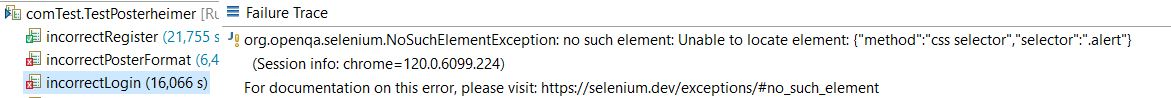
\includegraphics[width=\linewidth]{Slike/incorrectLoginFail}
				\caption{Prikaz pada ispitnog slučaja}
			\end{figure}
			
			
			
			U \textbf{četvrtom ispitnom slučaju} provjerena je funkcionalnost gumba za pristup konferenciji pri prijavi administratora. Predviđen rezultat je dozvoljen pristup konferenciji, te mogućnost dodavanja postera, fotografija i pokrovitelja. Ispitni slučaj je uspješan.
			
			\begin{lstlisting}
	  @Test
public void adminLogin() {
	System.setProperty("webdriver.chrome.driver", "src\\test\\java\\chromedriver\\chromedriver.exe");
	WebDriver driver = new ChromeDriver();
	driver.manage().timeouts().implicitlyWait(20, TimeUnit.SECONDS);
	// Vrijeme povecano zbog ucitavanja postera, koje je znatno sporije za administratora
	
	driver.get("https://posterheimer.onrender.com/");
	driver.manage().window().setSize(new Dimension(1552, 840));
	driver.findElement(By.cssSelector(".list-group-item:nth-child(2) > .float-end")).click();
	driver.findElement(By.id("username")).click();
	driver.findElement(By.id("username")).sendKeys("admin.test@mail.hr");
	driver.findElement(By.id("password")).click();
	driver.findElement(By.id("password")).sendKeys("Lozinka1");
	driver.findElement(By.cssSelector(".btn-primary")).click();
	driver.findElement(By.cssSelector(".conference-content")).click();
	driver.findElement(By.linkText("Posteri")).click();
	driver.findElement(By.cssSelector(".fa-solid")).click();
	driver.findElement(By.cssSelector(".btn-close")).click();
	driver.findElement(By.linkText("Fotografije")).click();
	driver.findElement(By.cssSelector(".image-container > img")).click();
	driver.findElement(By.cssSelector(".modal-title")).click();
	driver.findElement(By.cssSelector(".btn-close")).click();
	driver.findElement(By.linkText("Pokrovitelji")).click();
	driver.findElement(By.cssSelector(".fa-solid")).click();
	driver.findElement(By.cssSelector(".modal-title")).click();
	driver.findElement(By.cssSelector(".btn-close")).click();
	
	String redirURL = driver.getCurrentUrl();
	boolean comperRes = redirURL.contains("sponsors");
	if(comperRes) {
		System.out.println("Ostvaren rezultat");
	}
	driver.quit();
}
			\end{lstlisting}
			
			
	U \textbf{petom ispitnom slučaju} provjerena je funkcionalnost navigacijske trake. Predviđen rezultat je otvaranje stranice konferencije nakon klika na "Konferencija", stranice postera nakon klika na "Posteri", stranice za fotografije nakon klika na "Fotografije" i stranice pokrovitelja nakon klika na "Pokrovitelji". Ispitni slučaj je uspješan.
	
	\begin{lstlisting}
	  @Test
public void navBar() {
	System.setProperty("webdriver.chrome.driver", "src\\test\\java\\chromedriver\\chromedriver.exe");
	WebDriver driver = new ChromeDriver();
	driver.manage().timeouts().implicitlyWait(10, TimeUnit.SECONDS);	
	
	driver.get("https://posterheimer.onrender.com/");
	org.openqa.selenium.Dimension target = new  org.openqa.selenium.Dimension(1552, 840);
	driver.manage().window().setSize(target);
	
	driver.findElement(By.xpath("(//button[contains(text(),'Pristupi')])[2]")).click();
	// broj postaviti na mjesto konferencije u listi
	
	driver.findElement(By.id("username")).click();
	driver.findElement(By.id("username")).sendKeys("visitor.test@mail.hr");
	driver.findElement(By.id("password")).click();
	driver.findElement(By.id("password")).sendKeys("Lozinka1");
	driver.findElement(By.cssSelector(".btn-primary")).click();
	
	driver.findElement(By.linkText("Konferencija")).click();
	String redirURL = driver.getCurrentUrl();
	boolean comperRes = redirURL.contains("/conference");
	if(comperRes == true) {
		System.out.println("Pristupljeno konferenciji");
	} else {
		System.out.println("Error: konferencije");
	}
	
	driver.findElement(By.linkText("Posteri")).click();
	redirURL = driver.getCurrentUrl();
	comperRes = redirURL.contains("/posters");
	if(comperRes == true) {
		System.out.println("Pristupljeno posterima");
	} else {
		System.out.println("Error: posteri");
	}
	
	driver.findElement(By.linkText("Fotografije")).click();
	redirURL = driver.getCurrentUrl();
	comperRes = redirURL.contains("/photos");
	if(comperRes == true) {
		System.out.println("Pristupljeno fotografijama");
	} else {
		System.out.println("Error: fotografije");
	}
	driver.findElement(By.linkText("Pokrovitelji")).click();
	redirURL = driver.getCurrentUrl();
	comperRes = redirURL.contains("/sponsors");
	if(comperRes == true) {
		System.out.println("Pristupljeno pokroviteljima");
	} else {
		System.out.println("Error: pokrovitelji");
	}
	driver.quit();
}
	\end{lstlisting}
	
	U \textbf{šestom ispitnom slučaju} provjerena je funkcionalnost gumba za registraciju pri unosu adrese e-pošte netočnog formata. Sva ostala polja su točno ispunjena, a reCAPTCHA test je prošao. Predviđen rezultat je neuspješna registracija te obavijest o netočnom unosu. Ispitni slučaj je uspješan.
	Ispitni slučaj je neuspješan u slučaju CAPTCHA Image testa 

			\begin{lstlisting}
	  @Test
public void incorrectRegister() {
	System.setProperty("webdriver.chrome.driver", "src\\test\\java\\chromedriver\\chromedriver.exe");
	WebDriver driver = new ChromeDriver();
	JavascriptExecutor js = (JavascriptExecutor) driver;
	driver.manage().timeouts().implicitlyWait(10, TimeUnit.SECONDS);
	
	driver.get("https://posterheimer.onrender.com/");
	driver.manage().window().setSize(new Dimension(1552, 840));
	driver.findElement(By.cssSelector(".list-group-item:nth-child(2) > .float-end")).click();
	driver.findElement(By.cssSelector("form")).click();
	driver.findElement(By.id("username")).click();
	driver.findElement(By.id("username")).sendKeys("visitor.test@mail.hr");
	driver.findElement(By.id("password")).click();
	driver.findElement(By.id("password")).sendKeys("Lozinka1");
	driver.findElement(By.cssSelector(".btn-primary")).click();
	driver.findElement(By.linkText("Registracija")).click();
	js.executeScript("window.scrollTo(0,0)");
	driver.findElement(By.id("formIme")).click();
	driver.findElement(By.id("formIme")).sendKeys("TestIme");
	driver.findElement(By.id("formPrezime")).click();
	driver.findElement(By.id("formPrezime")).sendKeys("TestPrezime");
	driver.findElement(By.id("formBasicEmail")).click();
	driver.findElement(By.id("formBasicEmail")).sendKeys("email");
	driver.findElement(By.id("formBasicPassword")).click();
	driver.findElement(By.id("formBasicPassword")).sendKeys("lozinka");
	driver.findElement(By.cssSelector(".mb-3:nth-child(2) > #formBasicPassword")).click();
	driver.findElement(By.cssSelector(".mb-3:nth-child(2) > #formBasicPassword")).sendKeys("lozinka");
	driver.switchTo().frame(0);
	driver.findElement(By.cssSelector(".recaptcha-checkbox-border")).click();
	driver.switchTo().defaultContent();
	driver.findElement(By.cssSelector(".ml-2")).click();
	driver.findElement(By.cssSelector(".mx-2 > .mb-3:nth-child(1)")).click();
	driver.findElement(By.cssSelector(".mx-2 > .mb-3:nth-child(1)")).click();
	
	String redirURL = driver.getCurrentUrl();
	boolean comperRes = redirURL.contains("/register");
	if(comperRes == true) {
		System.out.println("Neuspjesna registracija");
	} else {
		System.out.println("Error");
	}
	
	driver.quit();
}	  
			\end{lstlisting}
			
		U \textbf{sedmom ispitnom slučaju} provjerena je funkcionalnost sučelja za dodavanje postera pri unosu datoteke netočnog formata. Prije dodavanja postera potrebna je prijava administratora. Predviđen rezultat je prikaz obavijesti "Izabrana datoteka nije PDF!". Rezultat je ostvaren.  
		
	\begin{lstlisting}
@Test
public void incorrectPosterFormat() {
	System.setProperty("webdriver.chrome.driver", "src\\test\\java\\chromedriver\\chromedriver.exe");
	WebDriver driver = new ChromeDriver();
	JavascriptExecutor js = (JavascriptExecutor) driver;
	File filepath = new File("src\\test\\java\\files\\example.pptx");
	
	
	driver.manage().timeouts().implicitlyWait(10, TimeUnit.SECONDS);
	
	
	driver.get("https://posterheimer.onrender.com/");
	driver.manage().window().setSize(new Dimension(1552, 840));
	driver.findElement(By.cssSelector(".list-group-item:nth-child(2) > .float-end")).click();	  
	
	driver.findElement(By.id("username")).click();
	driver.findElement(By.id("username")).sendKeys("admin.test@mail.hr");
	driver.findElement(By.id("password")).click();
	driver.findElement(By.id("password")).sendKeys("Lozinka1");
	driver.findElement(By.cssSelector(".btn-primary")).click();
	driver.findElement(By.linkText("Posteri")).click();
	driver.findElement(By.cssSelector(".fa-solid")).click();
	
	WebElement fileInput = driver.findElement(By.cssSelector("input[type=file]"));
	fileInput.sendKeys(filepath.getAbsolutePath());
	
	driver.findElement(By.name("imePoster")).click();
	driver.findElement(By.name("imePoster")).sendKeys("Krivi format");
	driver.findElement(By.name("imeAutor")).click();
	driver.findElement(By.name("imeAutor")).sendKeys("Ime");
	driver.findElement(By.name("prezimeAutor")).click();
	driver.findElement(By.name("prezimeAutor")).sendKeys("Prezime");
	driver.findElement(By.cssSelector("form")).click();
	driver.findElement(By.name("posterEmail")).click();
	driver.findElement(By.name("posterEmail")).sendKeys("test.poster@posterheimer.hr");
	driver.findElement(By.cssSelector(".btn")).click();
	
	WebElement alert = driver.findElement(By.cssSelector(".alert"));
	String errorMessage = alert.getText();
	if(errorMessage.contains("Izabrana datoteka nije PDF!")) {
		System.out.println("Prikaz prikladne obavijesti");
	} else {
		System.out.println("Error");
	}		
	
	driver.findElement(By.cssSelector(".alert")).click();
	driver.findElement(By.cssSelector(".btn-close")).click();
	
	
	driver.quit();
}
	\end{lstlisting}
			
			\subsection{Ispitivanje sustava}
			
			 \textit{Potrebno je provesti i opisati ispitivanje sustava koristeći radni okvir Selenium\footnote{\url{https://www.seleniumhq.org/}}. Razraditi \textbf{minimalno 4 ispitna slučaja} u kojima će se ispitati redovni slučajevi, rubni uvjeti te poziv funkcionalnosti koja nije implementirana/izaziva pogrešku kako bi se vidjelo na koji način sustav reagira kada nešto nije u potpunosti ostvareno. Ispitni slučaj se treba sastojati od ulaza (npr. korisničko ime i lozinka), očekivanog izlaza ili rezultata, koraka ispitivanja i dobivenog izlaza ili rezultata.\\ }
			 
			 \textit{Izradu ispitnih slučajeva pomoću radnog okvira Selenium moguće je provesti pomoću jednog od sljedeća dva alata:}
			 \begin{itemize}
			 	\item \textit{dodatak za preglednik \textbf{Selenium IDE} - snimanje korisnikovih akcija radi automatskog ponavljanja ispita	}
			 	\item \textit{\textbf{Selenium WebDriver} - podrška za pisanje ispita u jezicima Java, C\#, PHP koristeći posebno programsko sučelje.}
			 \end{itemize}
		 	\textit{Detalji o korištenju alata Selenium bit će prikazani na posebnom predavanju tijekom semestra.}
		 	
		 	Ispitivanje sustava provedeno je pomoću dodatka za preglednik Selenium IDE\footnote{https://www.selenium.dev/selenium-ide/}. JUnit ispitni slučajevi generirani su pomoću Selenium IDE ispitnih slučajeva.
		 	
		 	\textbf{Prvi ispitni slučaj} provjerava funkcionalnost brisanja korisnika. Prije brisanja korisnika potrebna je prijava registratora. Administrator briše određenog korisnika te se odjavljuje. Uspješnost brisanja korisnika provjeravamo pokušajem prijave izbrisanog korisnika. Očekivani rezultat je neuspješna prijava. Ispitni slučaj je uspješan.
		 	
		 	\begin{figure} [hbt!]
		 		\includegraphics[width=\linewidth]{Slike/deleteUser}
		 		\caption{Prikaz uspješnosti ispitnog slučaja}
		 	\end{figure}
		 	
		\begin{lstlisting}
  @Test
public void deleteUser() {
	driver.get("https://posterheimer.onrender.com/");
	driver.manage().window().setSize(new Dimension(1552, 840));
	driver.findElement(By.cssSelector(".list-group-item:nth-child(5) > .float-end")).click();
	{
		WebElement element = driver.findElement(By.cssSelector(".list-group-item:nth-child(5) > .float-end"));
		Actions builder = new Actions(driver);
		builder.moveToElement(element).perform();
	}
	{
		WebElement element = driver.findElement(By.tagName("body"));
		Actions builder = new Actions(driver);
		builder.moveToElement(element, 0, 0).perform();
	}
	driver.findElement(By.cssSelector(".mb-3:nth-child(1)")).click();
	driver.findElement(By.id("username")).click();
	driver.findElement(By.id("username")).sendKeys("admin.test@mail.hr");
	driver.findElement(By.cssSelector("form")).click();
	driver.findElement(By.id("password")).click();
	driver.findElement(By.id("password")).sendKeys("pass");
	driver.findElement(By.cssSelector(".btn-primary")).click();
	driver.findElement(By.id("user-dropdown")).click();
	driver.findElement(By.linkText("Korisnici")).click();
	driver.findElement(By.cssSelector(".list-group-item:nth-child(16) > .float-start")).click();
	driver.findElement(By.id("root")).click();
	driver.findElement(By.cssSelector(".list-group-item:nth-child(18) > .btn")).click();
	driver.findElement(By.id("user-dropdown")).click();
	driver.findElement(By.linkText("Odjava")).click();
	driver.findElement(By.cssSelector(".list-group-item:nth-child(5) > .float-end")).click();
	{
		WebElement element = driver.findElement(By.cssSelector(".list-group-item:nth-child(5) > .float-end"));
		Actions builder = new Actions(driver);
		builder.moveToElement(element).perform();
	}
	{
		WebElement element = driver.findElement(By.tagName("body"));
		Actions builder = new Actions(driver);
		builder.moveToElement(element, 0, 0).perform();
	}
	driver.findElement(By.id("username")).click();
	driver.findElement(By.id("username")).sendKeys("register2.");
	driver.findElement(By.id("username")).sendKeys("register2.email@mail.hr");
	driver.findElement(By.id("password")).click();
	driver.findElement(By.id("password")).sendKeys("pass");
	driver.findElement(By.cssSelector(".btn-primary")).click();
}
		\end{lstlisting}
		
\textbf{Drugi ispitni slučaj} provjerava funkcionalnost gumba za registraciju pri unosu podataka točnog formata. Tijekom registracije odabrana je opcija "Prikaz lozinke" te prođen CAPTCHA test. Rezultat ispitnog slučaja je uspješan.

\begin{figure} [hbt!]
	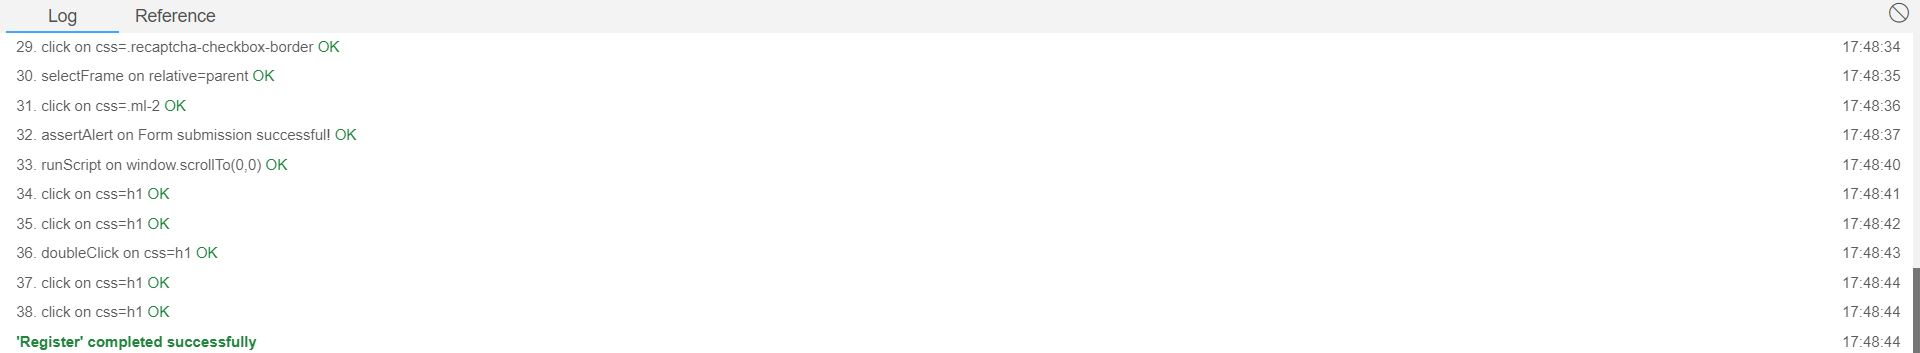
\includegraphics[width=\linewidth]{Slike/Register}
	\caption{Prikaz uspješnosti ispitnog slučaja}
\end{figure}

\begin{lstlisting}
	@Test
	public void register() {
		driver.get("https://posterheimer.onrender.com/");
		driver.manage().window().setSize(new Dimension(1552, 840));
		driver.findElement(By.cssSelector(".list-group-item:nth-child(5) > .float-end")).click();
		driver.findElement(By.id("username")).click();
		driver.findElement(By.id("username")).sendKeys("visitor.test@mail.hr");
		driver.findElement(By.id("password")).click();
		driver.findElement(By.id("password")).sendKeys("pass");
		driver.findElement(By.cssSelector(".btn-primary")).click();
		driver.findElement(By.cssSelector(".conference-content")).click();
		driver.findElement(By.cssSelector(".mx-auto:nth-child(1)")).click();
		driver.findElement(By.cssSelector(".card-text")).click();
		driver.findElement(By.linkText("Registracija")).click();
		js.executeScript("window.scrollTo(0,0)");
		driver.findElement(By.id("formIme")).click();
		driver.findElement(By.id("formIme")).sendKeys("TestIme");
		driver.findElement(By.id("formPrezime")).click();
		driver.findElement(By.id("formPrezime")).sendKeys("TestPrezime");
		driver.findElement(By.id("formBasicEmail")).click();
		driver.findElement(By.id("formBasicEmail")).click();
		driver.findElement(By.id("formBasicEmail")).sendKeys("register.email@mail.hr"); // promijeniti email za svaki test
		driver.findElement(By.id("formBasicPassword")).click();
		driver.findElement(By.id("formBasicPassword")).sendKeys("pass");
		driver.findElement(By.cssSelector(".mb-3:nth-child(2) > #formBasicPassword")).click();
		driver.findElement(By.cssSelector(".mb-3:nth-child(2) > #formBasicPassword")).sendKeys("pass");
		driver.findElement(By.cssSelector(".form-check")).click();
		driver.findElement(By.id("formShowPassword")).click();
		driver.findElement(By.id("formShowPassword")).click();
		driver.switchTo().frame(0);
		driver.findElement(By.cssSelector(".recaptcha-checkbox-border")).click();
		driver.switchTo().defaultContent();
		driver.findElement(By.cssSelector(".ml-2")).click();
		assertThat(driver.switchTo().alert().getText(), is("Form submission successful!"));
		js.executeScript("window.scrollTo(0,0)");
		driver.findElement(By.cssSelector("h1")).click();
		driver.findElement(By.cssSelector("h1")).click();
		{
			WebElement element = driver.findElement(By.cssSelector("h1"));
			Actions builder = new Actions(driver);
			builder.doubleClick(element).perform();
		}
		driver.findElement(By.cssSelector("h1")).click();
		driver.findElement(By.cssSelector("h1")).click();
	}
\end{lstlisting}

\textbf{Treći ispitni slučaj} provjerava funkcionalnost gumba za dodavanje konferencije. Prije dodavanja konferencije potrebna je prijava natkorisnika. Podaci vezani za korisnički račun natkorisnika uklonjeni su iz izvornog koda. Predviđen rezultat  je stvaranje nove konferencije. Ispitni slučaj je uspješan.

\begin{figure} [hbt!]
	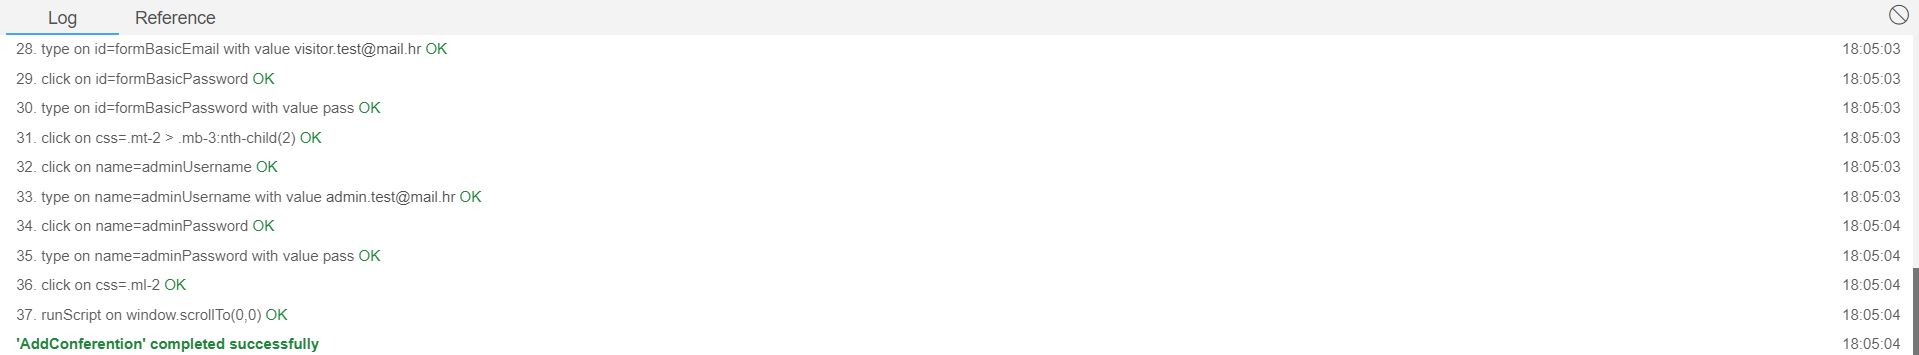
\includegraphics[width=\linewidth]{Slike/addConferention}
	\caption{Prikaz uspješnosti ispitnog slučaja}
\end{figure}

\begin{lstlisting}
	@Test
	public void addConferention() {
		driver.get("https://posterheimer.onrender.com/");
		driver.manage().window().setSize(new Dimension(1552, 840));
		driver.findElement(By.cssSelector(".fa-solid")).click();
		driver.findElement(By.id("username")).click();
		driver.findElement(By.id("username")).sendKeys("ime natkorisnika");
		driver.findElement(By.id("password")).click();
		driver.findElement(By.id("password")).sendKeys("lozinka natkorisnika");
		driver.findElement(By.cssSelector(".btn-primary")).click();
		driver.findElement(By.cssSelector(".fa-square-plus")).click();
		driver.findElement(By.id("formConferenceName")).click();
		driver.findElement(By.id("formConferenceName")).sendKeys("AutomaticTestKonferencija");
		driver.findElement(By.name("videoUrl")).click();
		driver.findElement(By.name("videoUrl")).sendKeys("https://www.youtube.com/watch?v=ScMzIvxBSi4&ab_channel=BenMarquezTX");
		driver.findElement(By.id("formConferenceCity")).click();
		driver.findElement(By.id("formConferenceCity")).sendKeys("Unska ");
		driver.findElement(By.id("formConferenceCity")).sendKeys("Unska 3");
		driver.findElement(By.id("formConferenceLocation")).click();
		driver.findElement(By.id("formConferenceLocation")).sendKeys("Zagreb");
		driver.findElement(By.id("formConferenceZipCode")).click();
		driver.findElement(By.id("formConferenceZipCode")).sendKeys("10000");
		driver.findElement(By.id("formDateStart")).click();
		driver.findElement(By.id("formDateStart")).sendKeys("2024-01-11T09:13");
		driver.findElement(By.id("formDateEnd")).click();
		driver.findElement(By.id("formDateEnd")).sendKeys("2024-01-14T09:13");
		driver.findElement(By.id("root")).click();
		driver.findElement(By.id("formBasicEmail")).click();
		driver.findElement(By.id("formBasicEmail")).sendKeys("visitor");
		driver.findElement(By.id("formBasicEmail")).sendKeys("visitor.test@mail.hr");
		driver.findElement(By.id("formBasicPassword")).click();
		driver.findElement(By.id("formBasicPassword")).sendKeys("pass");
		driver.findElement(By.cssSelector(".mt-2 > .mb-3:nth-child(2)")).click();
		driver.findElement(By.name("adminUsername")).click();
		driver.findElement(By.name("adminUsername")).sendKeys("admin.test@mail.hr");
		driver.findElement(By.name("adminPassword")).click();
		driver.findElement(By.name("adminPassword")).sendKeys("pass");
		driver.findElement(By.cssSelector(".ml-2")).click();
		js.executeScript("window.scrollTo(0,0)");
	}
\end{lstlisting}
		 	
		\textbf{Četvrti ispitni slučaj} provjerava funkcionalnost glasovanja. Prije samog glasovanja potrebna je prijava registriranog korisnika te odlazak na postere. Korisnik odabire jedan od postera, glasuje za njega te potvrđuje svoj glas. Zatim otvara drugi poster te više nema mogućnost glasovanja. Ispitni slučaj je uspješan.
		\begin{figure} [hbt!]
			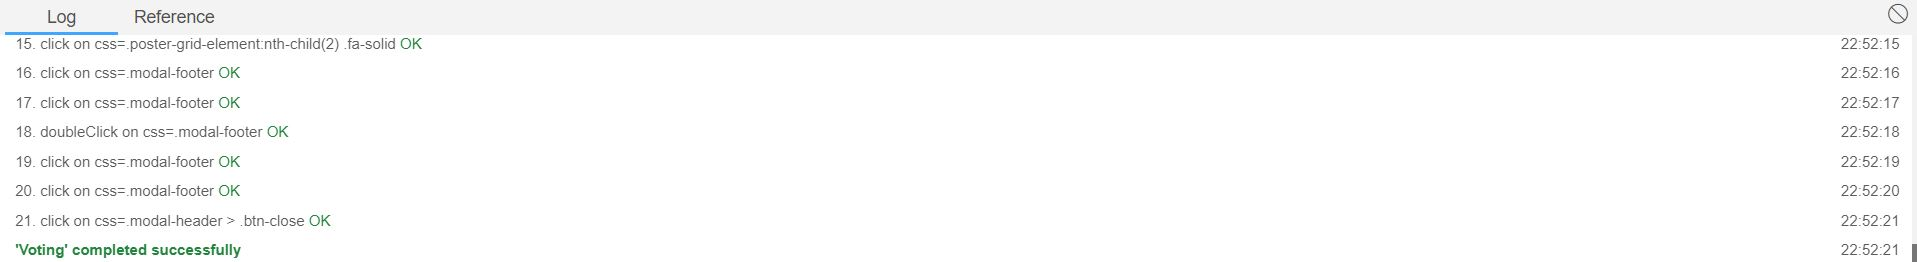
\includegraphics[width=\linewidth]{Slike/votingTest}
			\caption{Prikaz uspješnosti ispitnog slučaja}
		\end{figure}
		
		\begin{lstlisting}
@Test
public void voting() {
	driver.get("https://posterheimer.onrender.com/");
	driver.manage().window().setSize(new Dimension(1536, 824));
	driver.findElement(By.cssSelector(".list-group-item:nth-child(4) > .float-end")).click();
	driver.findElement(By.cssSelector("form")).click();
	driver.findElement(By.id("username")).click();
	driver.findElement(By.id("username")).sendKeys("register2.email@mail.hr");
	driver.findElement(By.id("password")).click();
	driver.findElement(By.id("password")).sendKeys("Lozinka1");
	driver.findElement(By.cssSelector(".btn-primary")).click();
	driver.findElement(By.linkText("Posteri")).click();
	driver.findElement(By.cssSelector(".poster-grid-element:nth-child(1) .fa-solid")).click();
	driver.findElement(By.cssSelector(".btn-success")).click();
	driver.findElement(By.cssSelector(".mx-2")).click();
	driver.findElement(By.cssSelector(".modal-header > .btn-close")).click();
	driver.findElement(By.cssSelector(".poster-grid-element:nth-child(2) .fa-solid")).click();
	driver.findElement(By.cssSelector(".modal-footer")).click();
	driver.findElement(By.cssSelector(".modal-footer")).click();
	{
		WebElement element = driver.findElement(By.cssSelector(".modal-footer"));
		Actions builder = new Actions(driver);
		builder.doubleClick(element).perform();
	}
	driver.findElement(By.cssSelector(".modal-footer")).click();
	driver.findElement(By.cssSelector(".modal-footer")).click();
	driver.findElement(By.cssSelector(".modal-header > .btn-close")).click();
}
		\end{lstlisting}
			
			\eject 
		
		
		\section{Dijagram razmještaja}
			
			\textbf{\textit{dio 2. revizije}}
			
			 \textit{Potrebno je umetnuti \textbf{specifikacijski} dijagram razmještaja i opisati ga. Moguće je umjesto specifikacijskog dijagrama razmještaja umetnuti dijagram razmještaja instanci, pod uvjetom da taj dijagram bolje opisuje neki važniji dio sustava.}
			 
			 \indent Dijagram razmještaja prikazuje odnos sklopovskih dijelova sustava međusobno i s programskim rješenjima koja su potrebna za korisnikovu interakciju s aplikacijom. Kao dio udaljene poslužiteljske infrastrukture postoje dva poslužiteljska računala: mrežni poslužitelj i poslužitelj baze podataka. Na mrežnom poslužitelju je aktivan proces programa aplikacije koji komunicira s bazom podataka koja je aktivna na vlastitom poslužitelju. Predviđeno je da korisnik koristi mrežni preglednik na vlastitom računalu za komunikaciju s aplikacijom na mrežnom poslužitelju.
			 
			 \begin{figure} [hbt!]
			 	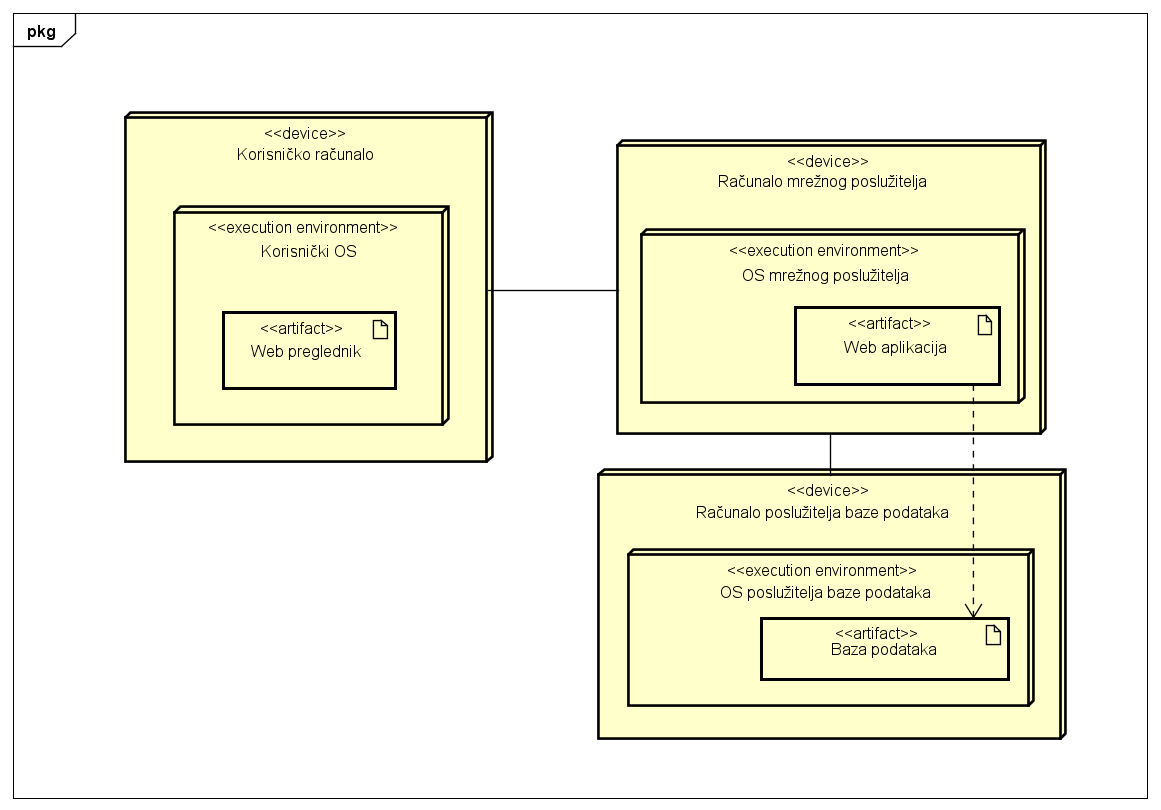
\includegraphics[width=\linewidth]{Slike/DeploymentDiagram}
			 	\caption{Dijagram razmještaja}
			 \end{figure}
			
			\eject 
		
		\section{Upute za puštanje u pogon}
		
			\subsubsection{Kreiranje baze podataka na serveru}
			Pri postavljanju projekta korištena je Render usluga na računalnom oblaku. Nakon izrade korisničkog računa možemo pristupiti opciji Dashboard, zatim odabiremo opciju "New +" - PostgreSQL. Unese se ime baze, a ostalo se automatski generira. Odabire se plan plaćanja (besplatna verzija uz više plaćenih), zatim Create. Time je baza kreirana. Sada ulaskom u dashboard imamo opciju "imebaze-db". Klikom na bazu ulazimo u prozor s informacijama o bazi od kojih su nam neke ključne za spajanje baze s \textit{backend} servisom.
			\newpage
			\begin{figure} [h]
				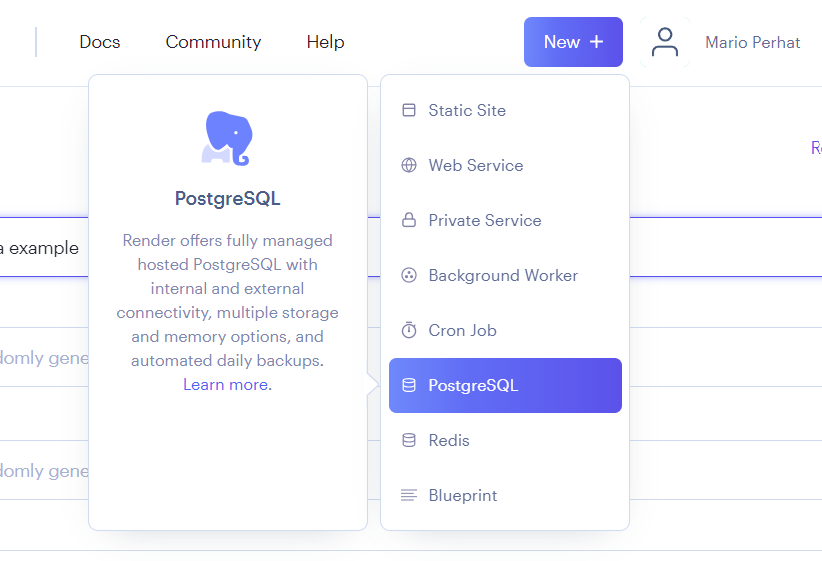
\includegraphics[width=\linewidth]{Slike/Dashboard-New-PostgreSQL}
				\caption{Dashboard-New-PostgreSQL}
			\end{figure}
			\newpage
			\begin{figure} [h]
				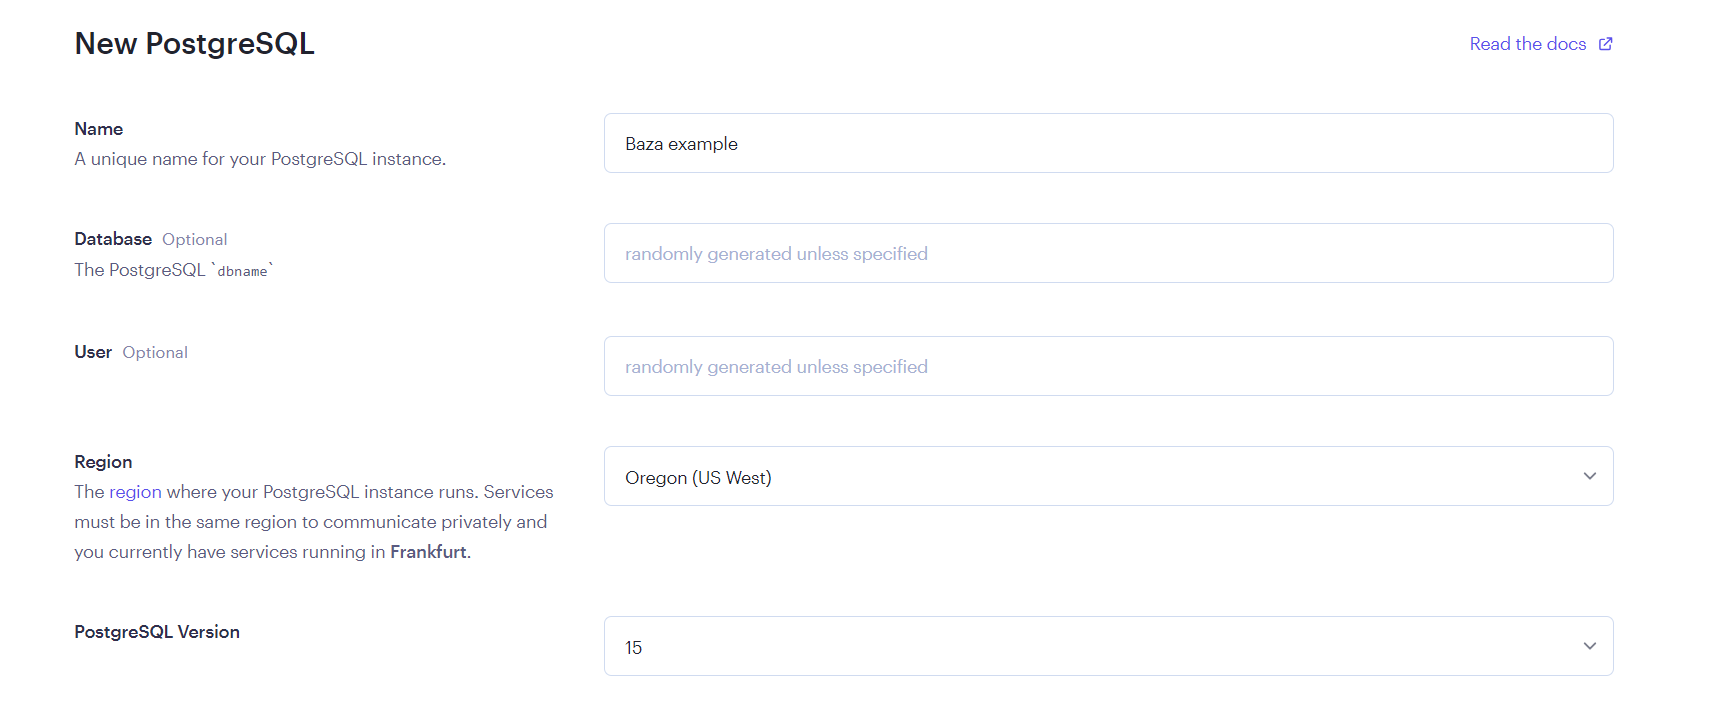
\includegraphics[width=\linewidth]{Slike/Izrada Baze Podataka}
				\caption{Izrada Baze Podataka}
			\end{figure}
			\newpage
			\begin{figure} [h]
				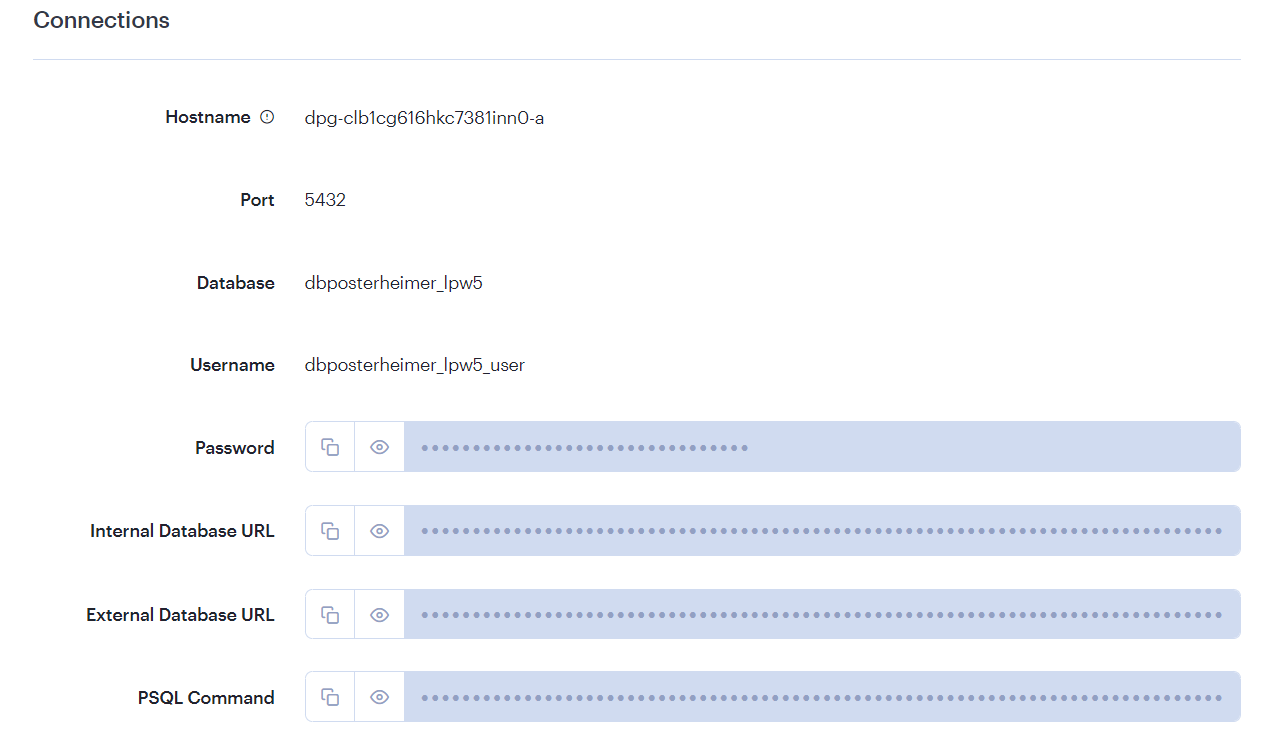
\includegraphics[width=\linewidth]{Slike/Info o Bazi Podataka}
				\caption{Info o Bazi Podataka}
			\end{figure}
			
			\newpage
			\subsubsection{Postavljanje backend servisa na server}
			Prije svega treba pripremiti \textit{backend} za puštanje na server. Dodaje se Dockerfile u direktorij "docker". Sličnim postupkom kao i za bazu, u Dashboard kliknemo "New +", zatim Web Service, nakon povezivanja git računa, dobije se pristup svim repozitorijima kojima račun ima pravo pristupa. Stisnuti "connect" kraj odgovarajućeg projekta.
			\begin{itemize}
			\item Postaviti ime servisa
			\item Root directory postaviti na IzvorniKod/posterheimer-backend
			\item Environment Docker
			\item Region postaviti na Frankfurt
			\item Na dnu proširiti advanced opciju
			\item Dodati potrebne environment varijable
			\item Stisnuti Create Web Service
			\end{itemize}
			Ako je sve dobro postavljeno, nakon što prođe potrebno vrijeme da se sve postavi na server, usluga bi trebala biti "live". 
			\newpage
			\begin{figure} [h]
				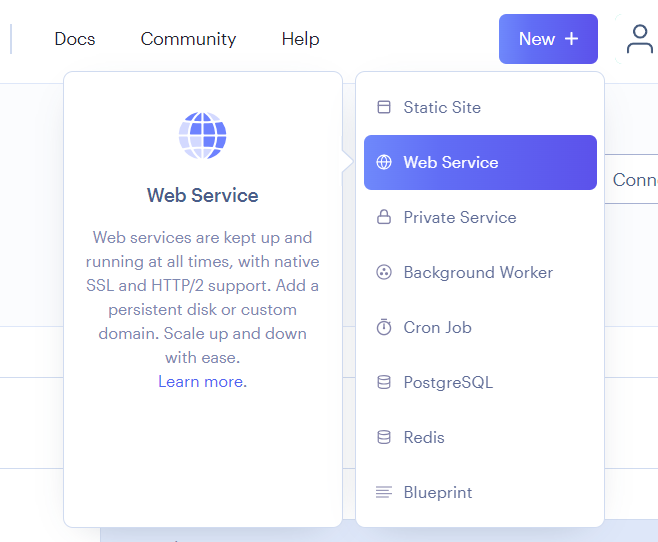
\includegraphics[width=\linewidth]{Slike/Dashboard-New-Web Service}
				\caption{Dashboard-New-Web Service }
			\end{figure}
			\newpage
			\begin{figure} [h]
				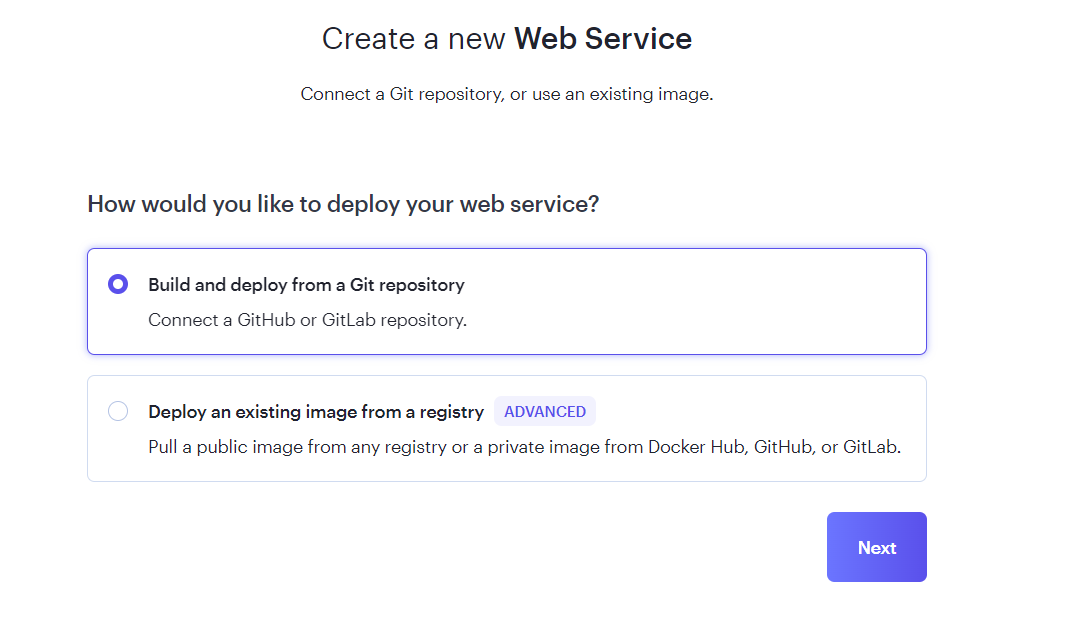
\includegraphics[width=\linewidth]{Slike/Stvaranje iz git repozitorija}
				\caption{Stvaranje iz git repozitorija}
			\end{figure}
			\newpage
			\begin{figure} [h]
				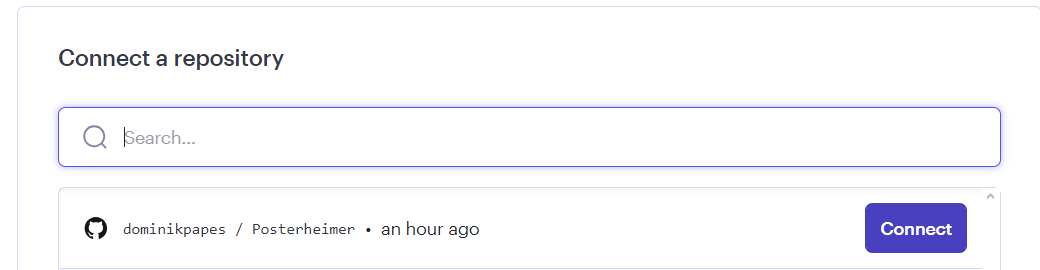
\includegraphics[width=\linewidth]{Slike/Spajanje s repozitorijem}
				\caption{Spajanje s repozitorijem}
			\end{figure}
			\newpage
			\begin{figure} [h]
				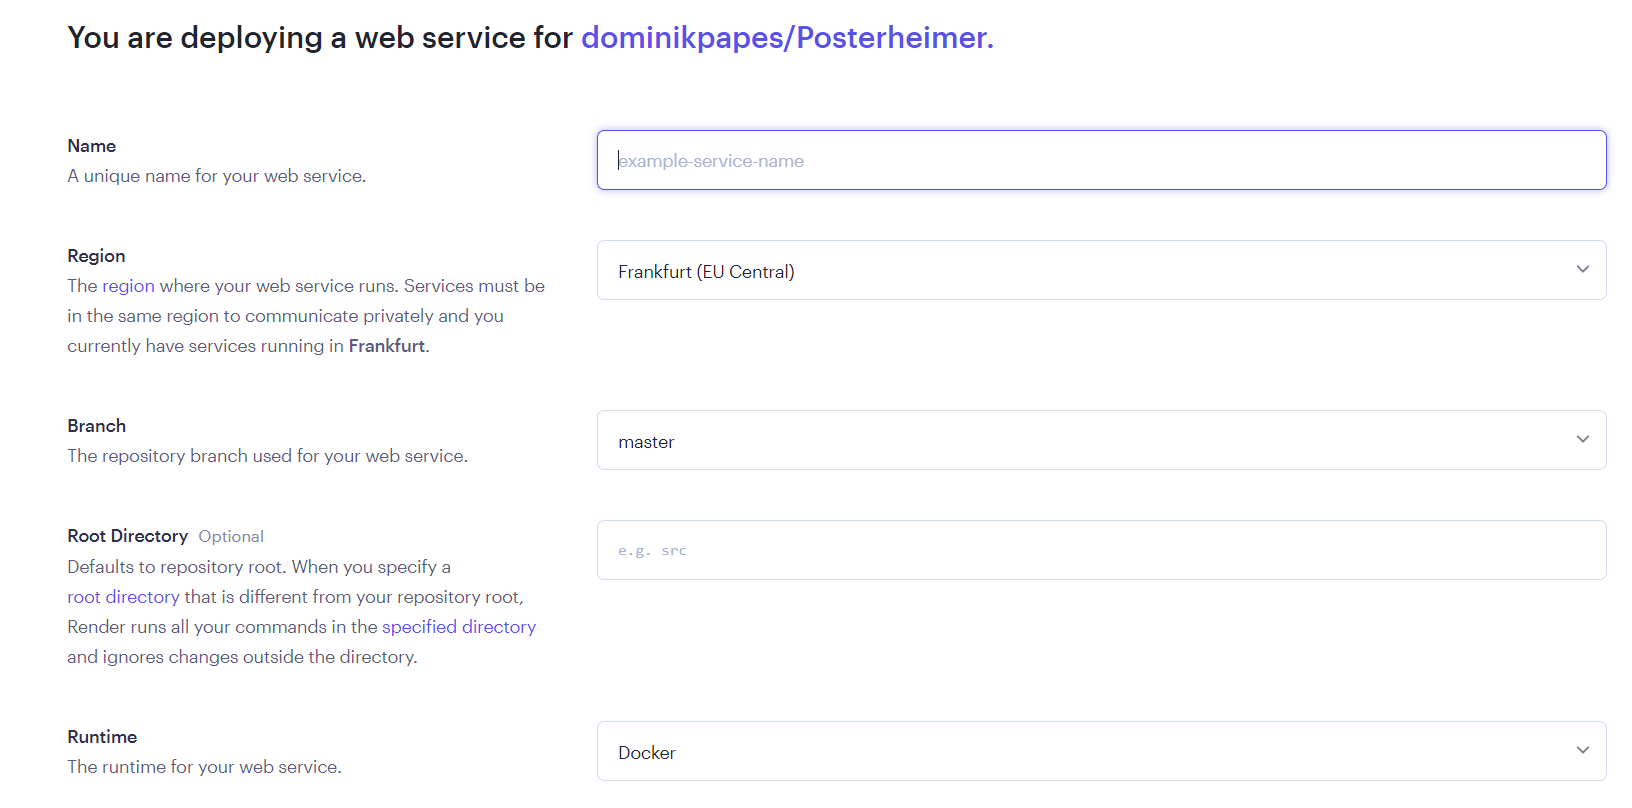
\includegraphics[width=\linewidth]{Slike/Polja za ispunjavanje}
				\caption{Polja za ispunjavanje}
			\end{figure}
			\newpage
			\begin{figure} [h]
				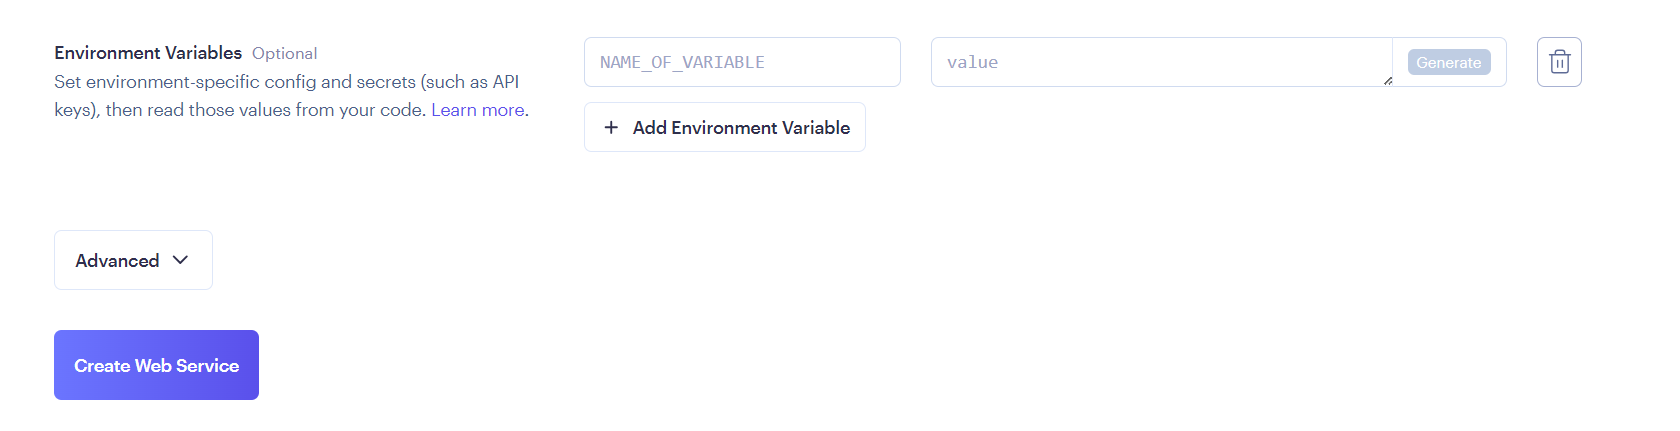
\includegraphics[width=\linewidth]{Slike/Dodavanje Environment varijabli}
				\caption{Dodavanje Environment varijabli}
			\end{figure}
			\newpage
			\begin{figure} [h]
				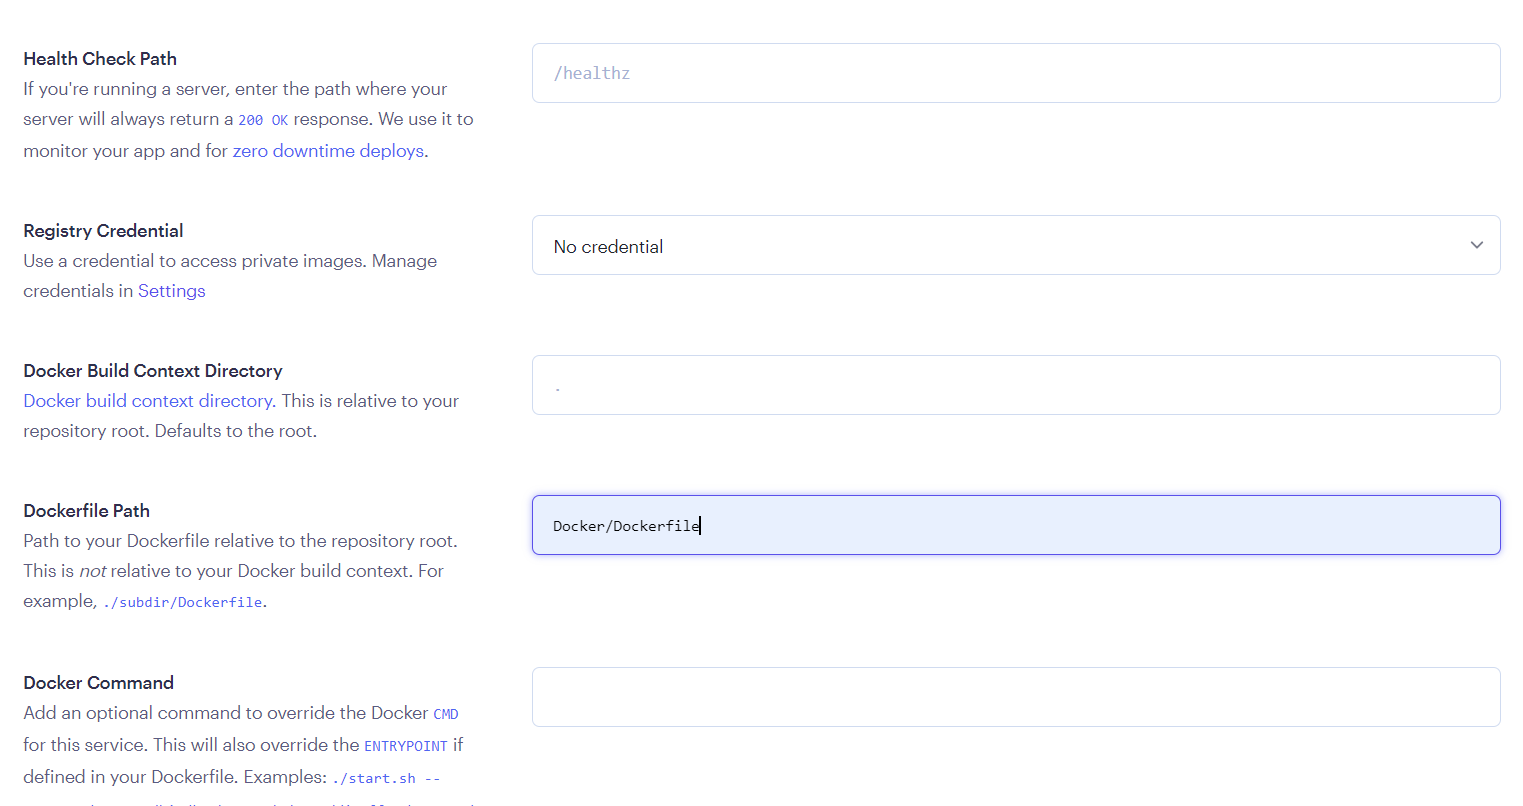
\includegraphics[width=\linewidth]{Slike/Advance-Docker path}
				\caption{Advance-Docker path}
			\end{figure}
			\newpage
			\begin{figure} [h]
				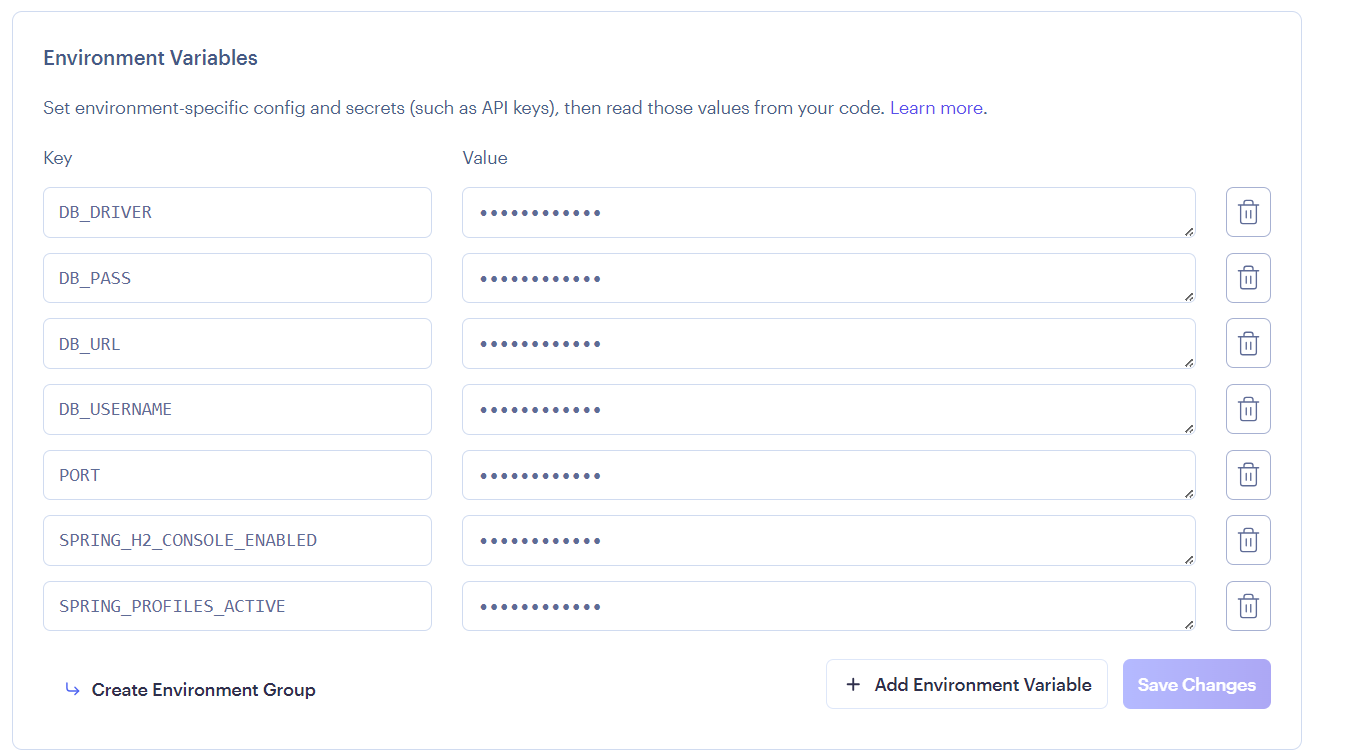
\includegraphics[width=\linewidth]{Slike/Environment varijable}
				\caption{Environment varijable }
			\end{figure}
			
			\subsubsection{Puštanje frontenda u pogon}
			Prije svega trebamo imati Github profil s repozitorijem koji sadrži naš kod. U ovom primjeru radi se o repozitoriju Posterheimer. Potom se trebamo prijaviti na Render s pripadajućim Github profilom. U Render Dashboardu odabiremo opciju "New" - "Web Service". 
			
			\newpage
			\begin{figure} [h]
			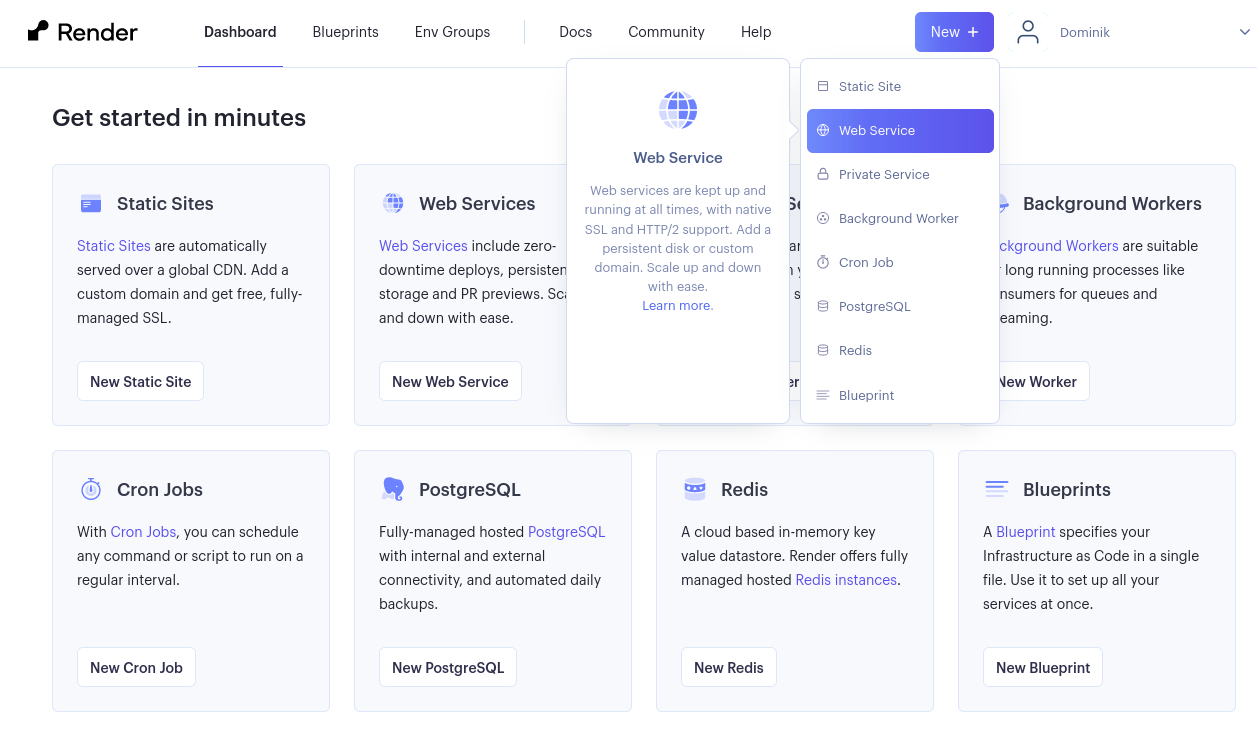
\includegraphics[width=\linewidth]{Slike/Render-Dashboard}
			\caption{Render Dashboard}
			\end{figure}
			
			\newpage
			U sljedećem izborniku odabiremo opciju "Build and deploy from a Git repository"
			
			\begin{figure} [h]
				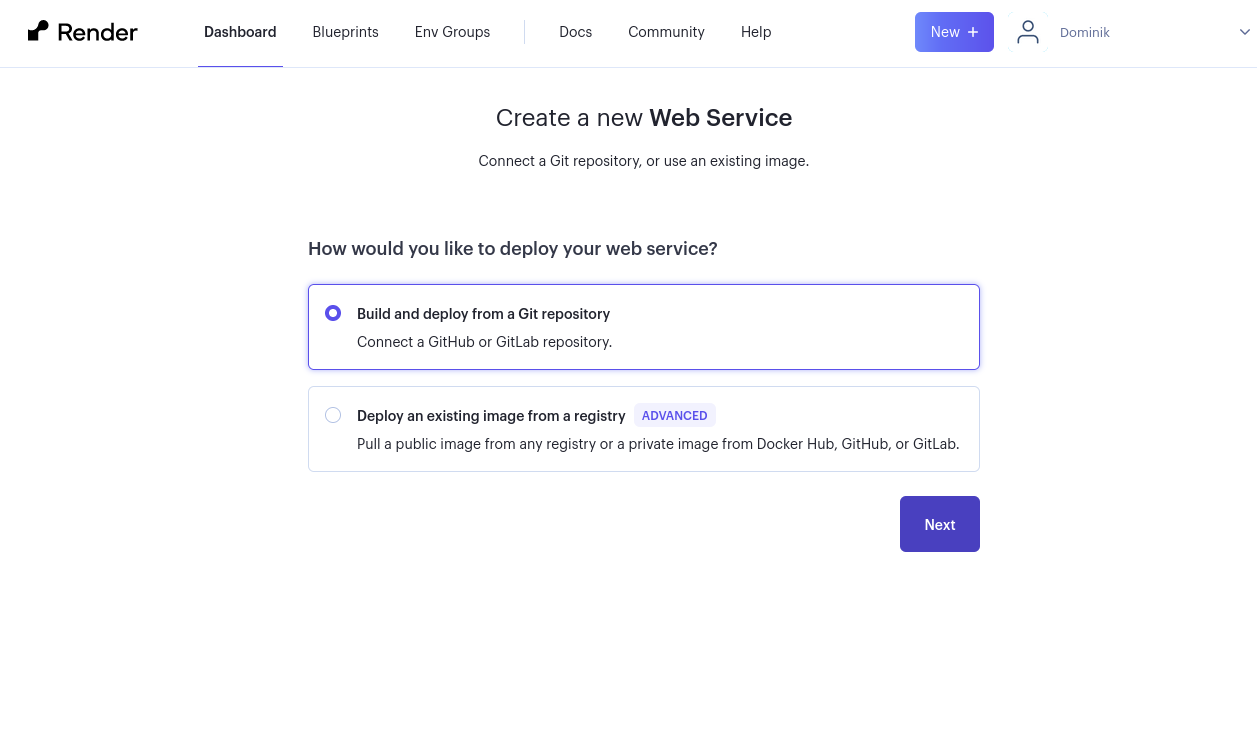
\includegraphics[width=\linewidth]{Slike/Build-and-deploy}
				\caption{Build and deploy}
			\end{figure}
			
			Iz izbornika izabiremo željeni repozitorij i odaberemo opciju "Connect". U sljedećem izborniku odaberemo željeno ime našeg servisa, regiju u kojoj će se servis pokretati, za europsko tržište odaberemo Frankfurt. Odabiremo granu s koje će se servis pokretati, u našem slučaju to je grana master. Specifično za pokretanje frontend koda želimo da se sve komande pokreću unutar direktorija IzvorniKod/posterheimer-frontend, stoga ćemo to upisati u polje Root directory. Runtime za naš servis je Node. Komanda izgradnje mora biti npm install \&\& npm run build. Kod samog pokretanja servisa treba se izvršiti naredba npm run start koju upisujemo u Start command polje.
			
			\newpage
			\begin{figure} [h]
			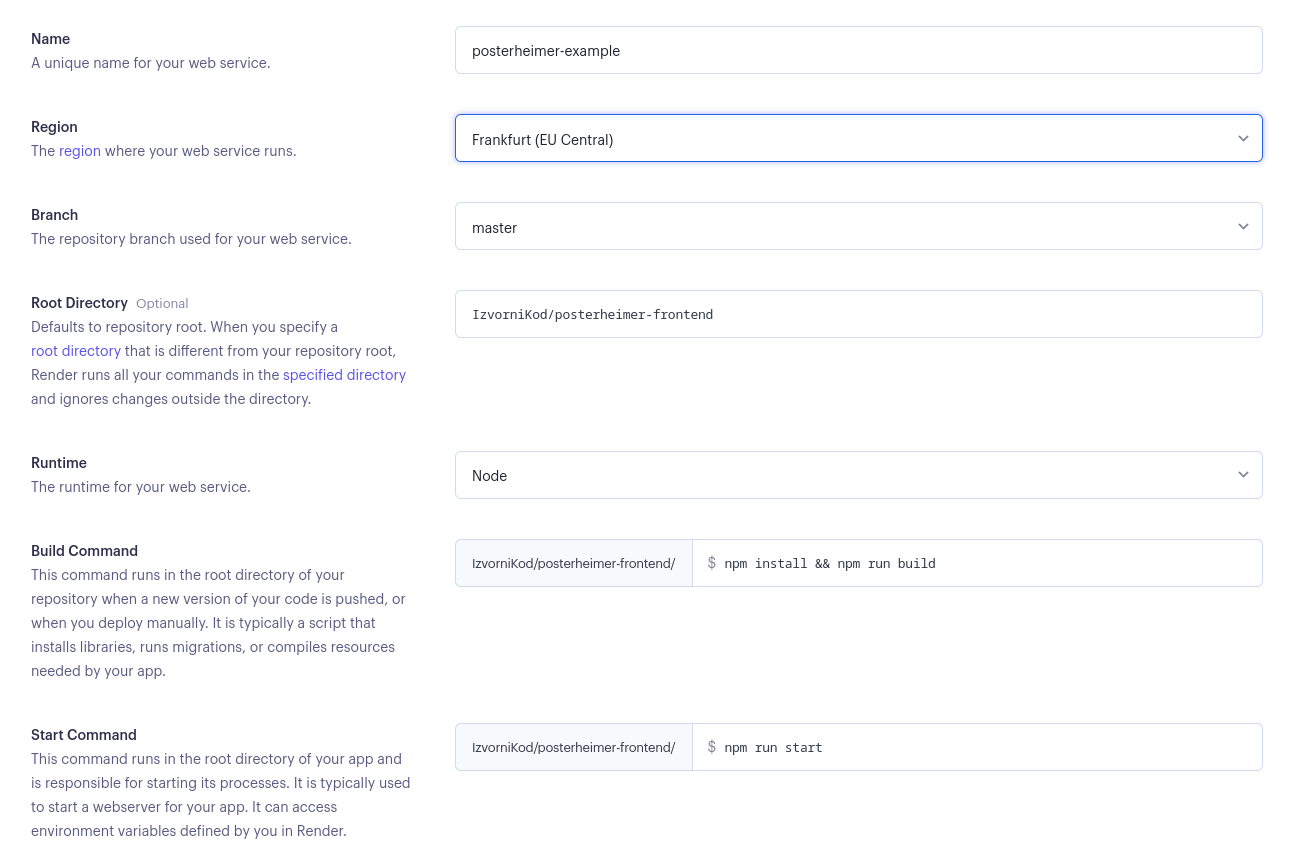
\includegraphics[width=\linewidth]{Slike/Run-Commands}
			\caption{Komande za pokretanje}
			\end{figure}
			
			Možemo odabrati vrstu instance našeg servisa, postoji besplatna opcija koja nudi najlošije performanse te koju ćemo koristiti  za potrebe ovog projekta.
			Potrebne su nam 3 varijable okoline, Environment variables.
			
			\begin{itemize}
				\item  API\_BASE\_URL = https://posterheimer-service.onrender.com - središnja ruta za sve API pozive prema serveru
				\item HOST = 0.0.0.0 - IP računala na kojem se izvodi servis
				\item  PORT = 3000 - port na kojem računalo sluša
			\end{itemize}
			
			Nakon što smo unijeli sve vrijednosti možemo kliknuti na "Create Web Service" gumb čime će se započeti puštanje aplikacije u pogon. Nakon kratkog čekanja trebali bismo vidjeti poruku "Your service is live!" nakon čega joj možemo pristupiti putem dodijeljenog linka, u ovom slučaju https://posterheimer-example.onrender.com/.
			
			\newpage
			\begin{figure} [h]
				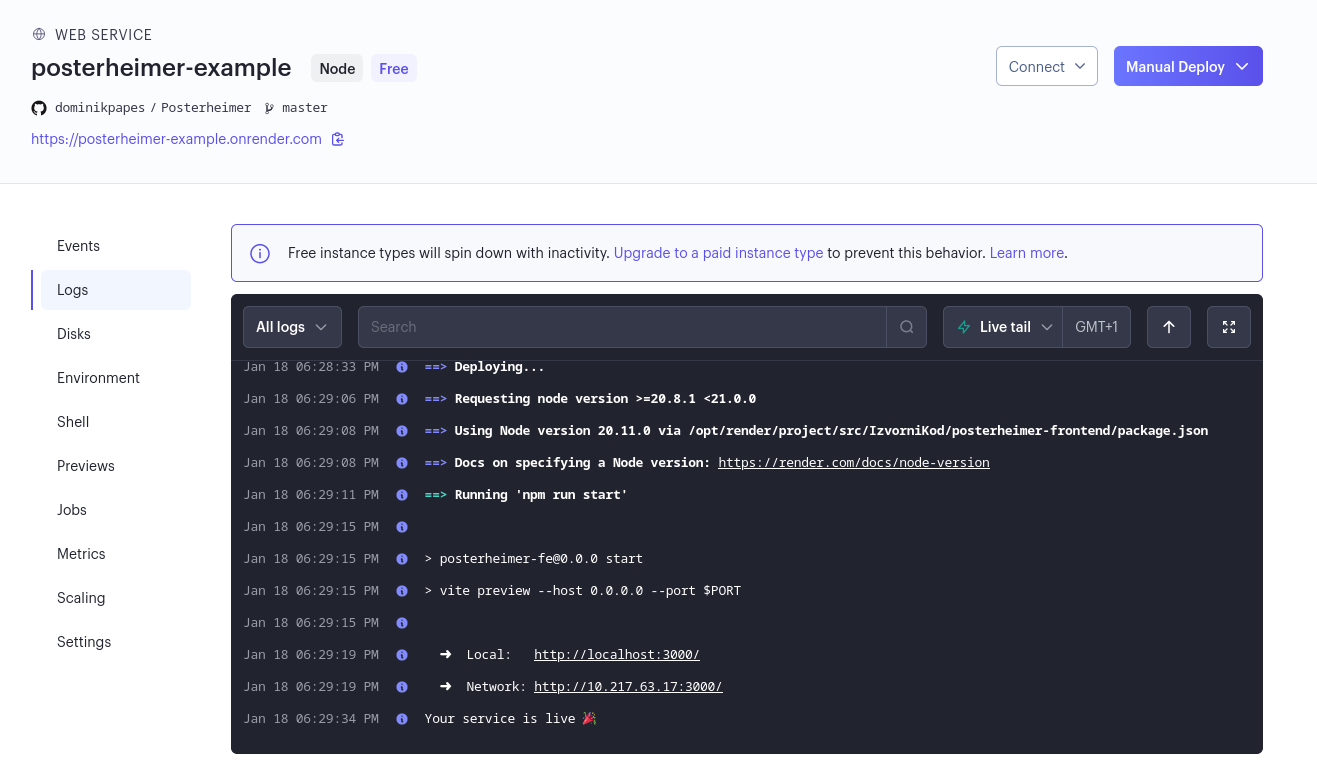
\includegraphics[width=\linewidth]{Slike/Frontend-Deployed}
				\caption{Aplikacija uspješno pokrenuta u pogon}
			\end{figure}
			\eject 
		\chapter{Zaključak i budući rad}
		
		\textbf{\textit{dio 2. revizije}}\\
		
		 \textit{U ovom poglavlju potrebno je napisati osvrt na vrijeme izrade projektnog zadatka, koji su tehnički izazovi prepoznati, jesu li riješeni ili kako bi mogli biti riješeni, koja su znanja stečena pri izradi projekta, koja bi znanja bila posebno potrebna za brže i kvalitetnije ostvarenje projekta i koje bi bile perspektive za nastavak rada u projektnoj grupi.}
		
		 \textit{Potrebno je točno popisati funkcionalnosti koje nisu implementirane u ostvarenoj aplikaciji.}
		 
		 Cilj projekta bio je razviti upotrebljivu aplikaciju od koje bi koristi imali organizatori događanja kao što su skupovi ili konvencije natjecateljskog tipa, gdje natjecatelji predstavljaju svoj rad posterom ili prezentacijom, a oni prisutni na događanju svojim glasom doprinose odluci o pobjedniku.
		 Tim koji je radio na aplikaciji sastojao se od šest članova, a rad na projektu trajao je sedamnaest tjedana, podijeljenih na dva dijela.
		 Završetak prvog dijela obilježilo je postavljanje potrebnih poslužitelja, te na njima uspostava početne baze podataka i početne inačice aplikacije. Prije toga se provelo prikupljanje i analiza zahtjeva, osmišljavanje funkcionalnosti aplikacije i dizajn arhitekture sustava, što je uključivalo odabir radnih okruženja i alata. Glavnina vremena ove etape iskoristila se na detaljan ispis obrazaca uporabe i crtanje dijagrama na temelju kojih bi se kasnije napisao kod.
		 S početkom drugog dijela razvoja, tim se podijelio u tri para, pri čemu su dva člana bila zadužena za prednji \textit{(engl. frontend)}, a dva za pozadinski \textit{(engl. backend)} dio koda, te dva člana za dovršavanje dokumentacije. U ovoj fazi se uglavnom stjecalo potrebno znanje i usavršavale se vještine za rad s odabranim radnim okvirima i knjižnicama, koje se tada koristilo za oblikovanje koda prisutnog u konačnom rješenju. Po uzoru na to rješenje pisao se nastavak dokumentacija, odnosno njezini dijelovi koji ovaj put služe kako bi opisali funkcionalnost programirane aplikacije.
		
		\eject 
		\chapter*{Popis literature}
		\addcontentsline{toc}{chapter}{Popis literature}
	 	
 		\textbf{\textit{Kontinuirano osvježavanje}}
	
		\textit{Popisati sve reference i literaturu koja je pomogla pri ostvarivanju projekta.}
		
		
		\begin{enumerate}
			
			
			\item  Programsko inženjerstvo, FER ZEMRIS, \url{http://www.fer.hr/predmet/proinz}
			
			\item  I. Sommerville, "Software engineering", 8th ed, Addison Wesley, 2007.
			
			\item  T.C.Lethbridge, R.Langaniere, "Object-Oriented Software Engineering", 2nd ed. McGraw-Hill, 2005.
			
			\item  I. Marsic, Software engineering book``, Department of Electrical and Computer Engineering, Rutgers University, \url{http://www.ece.rutgers.edu/~marsic/books/SE}
			
			\item  The Unified Modeling Language, \url{https://www.uml-diagrams.org/}
			
			\item  Astah Community, \url{http://astah.net/editions/uml-new}
		\end{enumerate}
		
		 
		
		
		\begingroup
		\renewcommand*\listfigurename{Indeks slika i dijagrama}
		%\renewcommand*\listtablename{Indeks tablica}
		%\let\clearpage\relax
		\listoffigures
		%\vspace{10mm}
		%\listoftables
		\endgroup
		\addcontentsline{toc}{chapter}{Indeks slika i dijagrama}
		
		
		
		\eject 
		
		\chapter*{Dodatak: Prikaz aktivnosti grupe}
		\addcontentsline{toc}{chapter}{Dodatak: Prikaz aktivnosti grupe}
		
		\section*{Dnevnik sastajanja}
		
		\textbf{\textit{Kontinuirano osvježavanje}}\\
		
		 \textit{U ovom dijelu potrebno je redovito osvježavati dnevnik sastajanja prema predlošku.}
		
		\begin{packed_enum}
			\item  sastanak
			
			\item[] \begin{packed_item}
				\item Datum: 18. listopada 2023.
				\item Prisustvovali: D.Papeš, F.Androić,A.Batić,V.Javornik,M.Perhat,D.Tomšić
				\item Teme sastanka:
				\begin{packed_item}
					\item  upoznavanje tima
					\item  dogovor načina komunikacije
				\end{packed_item}
			\end{packed_item}
			
			\item  sastanak
			\item[] \begin{packed_item}
				\item Datum: 23. listopada 2023.
				\item Prisustvovali: D.Papeš, F.Androić,A.Batić,V.Javornik,M.Perhat,D.Tomšić
				\item Teme sastanka:
				\begin{packed_item}
					\item  podjela članova u dvije podgrupe, prva će napraviti funkcionalne zahtjeve i obrasce uporabe, druga sekvencijske dijagrame i ostale zahtjeve
					\item  razmjena pitanja koje će grupa postaviti na laboratorijskim vježbama
				\end{packed_item}
			\end{packed_item}
			
			\item  sastanak
			\item[] \begin{packed_item}
				\item Datum: 1. studenoga 2023.
				\item Prisustvovali: D.Papeš, F.Androić,A.Batić,V.Javornik,M.Perhat,D.Tomšić
				\item Teme sastanka:
				\begin{packed_item}
					\item  dovršavanje obrazaca uporabe
					\item dogovaranje oko korisničkog sučelja aplikacije
				\end{packed_item}
			\end{packed_item}
			
			%
			
		\end{packed_enum}
		
		\eject
		\section*{Tablica aktivnosti}
		
			\textbf{\textit{Kontinuirano osvježavanje}}\\
			
			 \textit{Napomena: Doprinose u aktivnostima treba navesti u satima po članovima grupe po aktivnosti.}

			\begin{longtblr}[
					label=none,
				]{
					vlines,hlines,
					width = \textwidth,
					colspec={X[7, l]X[1, c]X[1, c]X[1, c]X[1, c]X[1, c]X[1, c]X[1, c]}, 
					vline{1} = {1}{text=\clap{}},
					hline{1} = {1}{text=\clap{}},
					rowhead = 1,
				} 
			
				\SetCell[c=1]{c}{} & \SetCell[c=1]{c}{\rotatebox{90}{\textbf{Dominik Papeš}}} & \SetCell[c=1]{c}{\rotatebox{90}{\textbf{Fran Androić }}} &	\SetCell[c=1]{c}{\rotatebox{90}{\textbf{Ante Batić }}} & \SetCell[c=1]{c}{\rotatebox{90}{\textbf{Valeria Javornik }}} &	\SetCell[c=1]{c}{\rotatebox{90}{\textbf{Mario Perhat }}} & \SetCell[c=1]{c}{\rotatebox{90}{\textbf{Dario Tomšić }}} \\  
				Upravljanje projektom 		& 3 &  &  &  & 1 &  \\ 
				Opis projektnog zadatka 	& 1 &  &  & 2 & 1 &  \\ 
				
				Funkcionalni zahtjevi       & 2 &  &  &  & 2 &  \\ 
				Opis pojedinih obrazaca 	& 3 & 3 & 3 & 3 & 3 & 3 \\ 
				Dijagram obrazaca 			&  &  &  &  &  &  \\ 
				Sekvencijski dijagrami 		&  &  &  &  &  &  \\ 
				Opis ostalih zahtjeva 		& 0.5 &  &  &  & 0.5 &  \\ 

				Arhitektura i dizajn sustava	 &  &  &  &  &  &   \\ 
				Baza podataka				&  &  &  &  &  &    \\ 
				Dijagram razreda 			&  &  &  &  &  &     \\ 
				Dijagram stanja				&  &  &  &  &  &   \\ 
				Dijagram aktivnosti 		&  &  &  &  &  &    \\ 
				Dijagram komponenti			&  &  &  &  &  &   \\ 
				Korištene tehnologije i alati 		&  &  &  &  &  &  \\ 
				Ispitivanje programskog rješenja 	&  &  &  &  &  &  \\ 
				Dijagram razmještaja			&  &  &  &  &  &  \\ 
				Upute za puštanje u pogon 		&  &  &  &  &  &  \\  
				Dnevnik sastajanja 			&  &  &  &  &  &  \\ 
				Zaključak i budući rad 		&  &  &  &  &  &  \\  
				Popis literature 			&  &  &  &  &  &   \\  
				&  &  &  &  &  &  \\ \hline 
				Učenje novih tehnologija & 1 &  &  &  & 5 &  \\ \hline 
				\textit{Dodatne stavke kako ste podijelili izradu aplikacije} 			&  &  &  &  &  &  \\ 
				\textit{npr. izrada početne stranice} 				&  &  &  &  &  &   \\  
				\textit{izrada baze podataka} 		 			&  &  &  &  &  &   \\  
				\textit{spajanje s bazom podataka} 							&  &  &  &  &  &   \\ 
				\textit{back end} 							&  &  &  &  &  &   \\  
				 							&  &  &  &  &  &  \\ 
			\end{longtblr}
					
					
		\eject
		\section*{Dijagrami pregleda promjena}
		
		\textbf{\textit{dio 2. revizije}}\\
		
		\textit{Prenijeti dijagram pregleda promjena nad datotekama projekta. Potrebno je na kraju projekta generirane grafove s gitlaba prenijeti u ovo poglavlje dokumentacije. Dijagrami za vlastiti projekt se mogu preuzeti s gitlab.com stranice, u izborniku Repository, pritiskom na stavku Contributors.}
		
	
		
				
	\end{document} %naredbe i tekst nakon ove naredbe ne ulaze u izgrađen dokument